\documentclass[msc,numbers]{coppe}
\usepackage{amsmath,amssymb}
\usepackage{hyperref}
\usepackage{algpseudocode}
\usepackage{algorithm}
\usepackage{graphicx}
\usepackage{caption}
\usepackage{subcaption}

\makelosymbols{}
\makeloabbreviations{}

\begin{document}
    \title{Event Localization in Computer Networks Using End-to-End
    Measurements}
    \foreigntitle{Event Localization in Computer Networks Using End-to-End
    Measurements}
    \author{Diego}{Ximenes Mendes}
    \advisor{Prof.}{Edmundo}{Albuquerque de Souza e Silva}{Ph.D.}

    %\examiner{Prof.}{Nome do Primeiro Examinador Sobrenome}{D.Sc.}
    %\examiner{Prof.}{Nome do Segundo Examinador Sobrenome}{Ph.D.}
    %\examiner{Prof.}{Nome do Terceiro Examinador Sobrenome}{D.Sc.}
    %\examiner{Prof.}{Nome do Quarto Examinador Sobrenome}{Ph.D.}
    %\examiner{Prof.}{Nome do Quinto Examinador Sobrenome}{Ph.D.}
    \department{PESC}
    \date{01}{2017}

    \keyword{Network Measurements}
    \keyword{Time Series}
    \keyword{Change Point Detection}
    \keyword{Machine Learning}

    \maketitle

    \frontmatter
    %\dedication{A algu\'em cujo valor \'e digno desta dedicat\'oria.}

    %\chapter*{Agradecimentos}

    \begin{abstract}
    Com o objetivo de melhor entender o desempenho de sua rede,
um grande tier-3 ISP brasileiro, em parceria com a UFRJ e a startup TGR,
estabeleceram um projeto para, atrav\'es de medidas fim-a-fim de QoS,
monitorar o servi\c{c}o prestado em um subconjunto dos seus clientes.

Nesse contexto, guiada pelas caracter\'isticas da rede do ISP, e do atual
processo de medi\c{c}\~ao, esta disserta\c{c}\~ao se prop\~oe a
avaliar a viabilidade de apenas utilizar m\'etricas fim-a-fim de QoS, e
traceroutes, para identificar e localizar eventos de rede. Um evento pode ser
interpretado como uma mudan\c{c}a no comportamento de um equipamento, que por
sua vez afeta a qualidade de servi\c{c}o percebida pelos usu\'arios,
como por exemplo, um defeito em um roteador.
O procedimento de localiza\c{c}\~ao define um conjunto de poss\'iveis
locais onde o evento pode ter acontecido.

Com esse prop\'osito, este trabalho prop\~oe um framework de an\'alise de dados,
que permite explorar mudan\c{c}as estat\'isticas nas s\'eries temporais de QoS
de diferentes clientes. Para detectar e localizar eventos, o mecanismo
correlaciona esses padr\~oes de altera\c{c}\~ao com traceroutes.
A fim de aumentar o
desempenho do sistema proposto, esta disserta\c{c}\~ao tamb\'em indica
poss\'iveis melhorias na atual metodologia de medi\c{c}\~ao.

    \end{abstract}

    \begin{foreignabstract}
    To better understand the performance of it's own network, a major
Tier-3 Brazilian ISP, in partnership with UFRJ and the startup TGR,
established a project to monitor the service provided to a subset
of it's customers.

In this context, guided by the specific ISP's network's charateristics
and the current measurement process,
this dissertation aims to check the viability of
only using end-to-end QoS measures, and traceroutes,
to identify and localize network events. An event can be interpreted as a
behavioral change in a network equipment, that affect the quality of service
perceived by the end-users,
such as a router failure. The localization procedure defines a set of
feasible locations where the event could have happened.

For such purpose, this work proposes a data analytics framework, which is able
to track statistical changes in the QoS time series of different
clients.
To detect and localize events, the mechanism correlates these modification
patterns with traceroutes.
In order to increase the system's performance,
this dissertation also indicates possible improvements in the current
measurement methodology.

    \end{foreignabstract}

    \tableofcontents
    \listoffigures
    \listoftables
    \printlosymbols{}
    \printloabbreviations{}

    \mainmatter{}

    \chapter{Introduction}

To better understand the performance of it's own network, a major
tier-3 Brazilian \gls*{isp}, in partnership with \gls*{ufrj} and a startup
incubated at this university,
established a project to monitor the service provided to a subset
of it's customers.

Considering the \gls*{isp}'s cable-television infrastructure,
which runs \gls*{docsis},
\gls*{qos} metrics are gathered through a software placed at home routers
connected to cable modems. This software is responsible to perform end-to-end
measurements against servers strategically located by the \gls*{isp}.

In this context, guided by the specific \gls*{isp}'s network's characteristics,
and the current measurement process,
this dissertation aims to check the viability of
only using end-to-end \gls*{qos} measures, and traceroutes,
to identify and localize network events. An event can be interpreted as a
behavioral change in a network equipment, that affect the quality of service
perceived by the end-users,
such as a router failure. The localization procedure defines a set of
feasible locations where the event could have happened.

For such purpose, this work proposes a data analytics framework, which is able
to track statistical changes in the \gls*{qos} time series of different
clients.
To detect and localize events, the mechanism correlates these modification
patterns with traceroutes.
In order to increase the system's performance,
this dissertation also indicates possible improvements in the current
measurement methodology.

\section{Contributions}

Considering the specific \gls*{isp}'s network topology,
and the already implemented
measurement process, next is listed this dissertation's main contributions.

\begin{itemize}
\item
A data analytics procedure, that only uses the available end-to-end \gls*{qos}
measurements, and traceroutes, to detect and localize network events.

\item
A list of possible improvements in the measurement methodology currently
employed by the startup, in order to enhance the proposed system's performance.

\end{itemize}

\section{Dissertation Outline}

Chapter~\ref{chap:literature_review} consists of a literature review, that
describes three previous systems that use
end-to-end measurements to localize network events.
To track statistical changes in the time series, the current
work deploys change point detection methods. Then,
Chapter~\ref{chap:change_point_detection} presents several of these algorithms,
including the developed strategies to better handle the end-to-end \gls*{qos} data
characteristics.
In Chapter~\ref{chap:methodology} is detailed the measurement methodology and
the proposed data analytics workflow.
Chapter~\ref{chap:results} presents several results when the proposed pipeline
was applied to real data.
Finally, Chapter~\ref{chap:conclusion} concludes the work and
points future directions.

The code developed to support this dissertation is available at
\url{https://bitbucket.org/diegoximenes/master_thesis}.
Unfortunately, due to a \gls*{nda},
the data used in this project can not be open sourced.

    \chapter{Literature Review of Change Point Detection} 

- Here the change point problem will be "defined", including offline and online versions.
- we deal with univariate unevenly time series. Explain that some methods can be expanded no multivariate
- unknow number of change points
- we disconsider changes in periodicity

\section{Notation}

In this work an univariate time series composed of $n$ points is defined by two vectors: $\mathbf{x} = (x_{1}, ..., x_{n})$ and $\mathbf{y} = (y_{1}, ..., y_{n})$. The value $y_{i}$ indicates the $i-$th sampled value and $x_{i}$ indicates the associated sample time. It is assumed that the points are sorted by time, that is, $x_{i - 1} < x_{i}$ for $i = 1, ..., n$. Since we consider unevenly time series $x_{i} - x_{i - 1}$ can be different for different $i$ values. For $s \ge t$ the following convention is adopted $\mathbf{y}_{s:t} = (y_{s}, ..., y_{t})$.

The presence of $k$ change points indicates that the data is splitted into $k+1$ segments, also called windows. Let $\tau_{i}$ indicate the $i-$th change point for $i=1,...,k$. Let $\tau_{0} = 0$ and $\tau_{k + 1} = n$. Then, the $i-$th segment is defined by $\mathbf{y}_{\tau_{i - 1} + 1 : \tau_{i}}$, assuming that $\tau_{i - 1} < \tau_{i}$ for $i = 0, ..., k + 1$. Therefore $\boldsymbol \tau = (\tau_{0}, ..., \tau_{k + 1})$.

\section{Sliding Window Techniques}

Mainly a change point detection algorithm aim to find $k$ and $\boldsymbol \tau$.

Describe sliding window techniques in change point detection. Describe how two windows can be compared. Probably this technique will not be part of my solution, but I will write about it since is the simplest and most intuitive solution.

\section{Combinatorial Optimization Model}  

\subsection{Constrained Case}

Given a fixed value of $k$, one approach is to define a cost function that measure the homogeneity of a segment and therefore choose the change points that globally optimize this homogeneity. Let the cost of the $i$-th segment be defined as $C(y_{\tau_{i - 1} + 1 : \tau_{i}})$. The cost of a segmentation is then $\sum \limits_{i = 1}^{k + 1} C(y_{\tau_{i - 1} + 1 : \tau_{i}})$.

A commom choice for function $C$ is the MSE (Mean Squared Error) which can capture changes in the mean. Another usual approach is to consider a distributin model and use the negative maximum log-likelihood. The latter can capture changes in mean and variance, also considers that data within a segment is iid. Therefore, given a fixed $k$, the optimal segmentation is obtained through the following optimization problem: 

\begin{equation}
    F_{k, n} = \min_{\boldsymbol \tau_{1 : k}} \sum \limits_{i = 1}^{k + 1} C(y_{\tau_{i - 1} + 1 : \tau_{i}})
\end{equation}

This problem can be solved using dynamic programming:

\begin{equation}
    F_{k, t} = 
    \begin{cases}
        0, & \text{if } k = 0 \text{ and } t = 0 \\
        \infty, & \text{if } k = 0 \text{ and } t > 0 \\
        \displaystyle \min_{s \in \{0, ..., t - 1\}} \left[ F_{k - 1, s} + C(y_{s + 1 : t}) \right], & \text{ otherwise}
    \end{cases}
\end{equation}

Given that function $C$ can be evaluated in $O(1)$, the overal time complexity of this algorithm is $O(k n^2)$.

\subsection{Segment Cost Function}

Several segment cost functions can be evaluated in $O(1)$ after a preprocessing phase. Next is provided the procedures to achieve this efficiency using MSE, negative maximum log-likelihood of normal and exponential distributions.

\subsubsection{MSE}

Let $\mu_{s, t}$ the mean value of the segment $\mathbf{y}_{s : t}$:

\begin{equation}
    \mu_{s, t} = \frac{\sum \limits_{i = s}^{t} y_{i}}{t - s + 1}
\end{equation}

Then, the $MSE(\mathbf{y}_{s : t})$ is defined as:

\begin{equation}
    \begin{aligned}
        MSE(\mathbf{y}_{s : t}) = \frac{\sum \limits_{i = s}^{t} (y_{i} - \mu_{s, t})^{2}}{t - s + 1} \\
        = \frac{\sum \limits_{i = s}^{t} (y_{i}^{2} - 2 y_{i} \mu_{s, t} + \mu_{s, t}^{2})}{t - s + 1} \\
        = \frac{\sum \limits_{i = s}^{t} y_{i}^{2} - 2 \mu_{s, t} \sum \limits_{i = s}^{t} y_{i} + (t - s + 1) \mu_{s, t}^{2}}{t - s + 1} \\
    \end{aligned}
\end{equation}

Let $S_{i} = \sum \limits_{j = 0}^{i} y_{j}$, that is, $\mathbf{S}$ represents the prefix sum of $\mathbf{y}$ for different indexes. $\mathbf{S}$ can be computed in $O(n)$ with the following dynamic programming procedure: 

\begin{equation}
    S_{i} = 
    \begin{cases}
        0, & \text{if } i = 0 \\
        S_{i - 1} + y_{i}, & \text{otherwise}
    \end{cases}
\end{equation}

Let $Q_{i} = \sum \limits_{j = 0}^{i} y_{j}^{2}$. As with $\mathbf{S}$, $\mathbf{Q}$ can be computed in $O(n)$: 

\begin{equation}
    Q_{i} = 
    \begin{cases}
        0, & \text{if } i = 0 \\
        Q_{i - 1} + y_{i}^{2}, & \text{otherwise}
    \end{cases}
\end{equation}

Given that $\mathbf{S}$ and $\mathbf{Q}$ are previously computed, it is possible to evaluate the following equations in $O(1)$: 

\begin{equation}
    \label{mean_o1}
    \mu_{s, t} = \frac{S_{t} - S_{s - 1}}{t - s + 1}
\end{equation}

\begin{equation}
    \label{prefixsum1_o1}
    \sum \limits_{i = s}^{t} y_{i} = S_{t} - S_{s - 1}
\end{equation}

\begin{equation}
    \label{prefixsum2_o1}
    \sum \limits_{i = s}^{t} y_{i}^{2} = Q_{t} - Q_{s - 1}
\end{equation}

With equations \ref{mean_o1} \ref{pre}

\subsubsection{Negative Log-Likelihood of Normal Distribution}
\subsubsection{Negative Log-Likelihood of Exponential Distribution}

- degenerate distribution

\subsection{Penalized Case}

When the number of change points is unknown.

\subsection{Pruning}
- heuristics

\section{Bayesian Inference}
I will erase this section if I don't use bayesian inference. Describe Fearnheard (offline) and MacKay (online) solutions. Say that there are other versions.

\section{HMM}
I will not describe HMM algorithms (viterbi, baum welch, etc), I will only describe how HMM have been used in change point detection. Describe Left-Right HMM, full HMM, and Regularized HMM in this problem.

\section{Other Algorithms}
Only cite other used algorithms and say why I chose the previous one to analyse.

\section{Performance Evaluation}
  Describe how datasets are constructed in literature. Describe how an algorithm output is evaluated.


    \chapter{Change Point Detection} 

A change point detection algorithm is concerned to identify points in time where the statistical properties of a time series have changed. This problem have a broad application in different knowledge fields, and in general, the algorithms performance are closely related with the input characteristics. Also, if the latent information of the procedures that generated a time series is missing, the target statistical properties can be considered subjective, bringing difficulties not only in the detection phase but also in the problem formalization.

In this context this chapter specifies the problem and briefly discusses several change point detection algorithms. The literature of this area is extensive, and it is common to find methods that presents a poor performance due to a variety of reasons, such as they are too specific or because the mechanisms were only analyzed through theoretical aspects. Therefore, it was chosen a set of methods that can provide a good practical and theoretical perspective, and also flexibility to insert adaptations that can better handle some input peculiarities. Furthermore, through this chapter is exposed several obstacles when dealing with real data, and some adopted solutions which are not described in literature.

\section{Problem Definition}

The problem can be categorized in offline or online. In the offline version, to decide if a specific point at time $t$ is a change point the solver has available the whole time series, including past and future information on $t$. In the other hand, in the online version the information is available up to time $t$. The choice between these options is defined by the application domain, in some cases data are processed in real time and the change points should be detected as soon as possible, but in others the changes are identified by historical purposes and offline algorithms can be used. 

It is intuitive that the offline case is more robust, since there are more information to make a classification. In practice, to increase the statistical confidence of a decision the online definition is relaxed, and to decide if a point at time $t$ is a change point it is possible to use data up to a small window in the future of $t$, which in real time processing means that the application should wait until more data are available. This trick plays a trade-off between minimizing the time to detect a change and correctly classify a point. Therefore, in some cases, the online version can be transformed in the offline case by only modifying the input availability. 

In this work it is considered the following input and change points characteristics, which were defined considering the final application scenario:
\begin{itemize}
    \item Univariate time series. However, it is possible to extend several methods presented here to deal with multivariate data.
    \item Unevenly time series, that is, data is not regularly sampled in time.
    \item Time series with different lengths.
    \item Unknown number of change points.
    \item Different number of points between change points.
    \item Focus on changes in the underlying mean and distribution, disregarding other kinds of changes such as in periodicity.
    \item Outliers are not considered statistical changes.
    \item There is no latent information of the time series.
    \item It is considered the online and offline options.
\end{itemize}

\section{Notation}

An univariate time series composed of $n$ points is defined by two vectors, $\mathbf{x} = (x_{1}, ..., x_{n})$ and $\mathbf{y} = (y_{1}, ..., y_{n})$. The value $y_{i}$ indicates the $i$-th sampled value and $x_{i}$ indicates the associated sample time. It is assumed that the points are sorted by time, that is, $x_{i - 1} < x_{i}$ for $i = 2, ..., n$. Since unevenly time series is considered, $x_{i} - x_{i - 1}$ can be different for different $i$ values. For $s \ge t$ the following convention is adopted: $\mathbf{y}_{s:t} = (y_{s}, ..., y_{t})$.

The presence of $k$ change points implies that data is split into $k+1$ segments, also called windows. Let $\tau_{i}$ indicates the $i$-th change point for $i=1,...,k$. Also let $\tau_{0} = 0$, $\tau_{k + 1} = n$ and $\boldsymbol \tau = (\tau_{0}, ..., \tau_{k + 1})$. Then, the $i$-th segment is defined by $\mathbf{y}_{\tau_{i - 1} + 1 : \tau_{i}}$, assuming that $\tau_{i - 1} < \tau_{i}$ for $i = 1, ..., k + 1$.

Through the previous definitions, change point detection algorithms mainly aim to find both $k$ and $\boldsymbol \tau$.

\section{Sliding Windows}

Sliding windows techniques use two sliding windows over the time series, and reduce the problem of detecting change points to the problem of testing whether data from the segments were generated by different distributions. One approach is to consider a distance metric between two empirical distributions as the base to infer the change points. Letting $d(\mathbf{a}, \mathbf{b})$ be the distance between two empirical distributions defined by the windows $\mathbf{a}$ and $\mathbf{b}$, and considering windows of length $m$, the Algorithm~\ref{alg:sliding_windows} presents a simple sliding windows method.

\begin{algorithm}
    \caption{Sliding Windows}
    \label{alg:sliding_windows}
	\begin{algorithmic}[1]
		\State $i \gets 1$
		\While{$i + 2 m - 1 \leq n$}
             \If{$d(\mathbf{y}_{i : i + m - 1}, \mathbf{y}_{i + m : i + 2m - 1}) > \alpha$}
                \State Report $i + m - 1$ as a change point
		        \State $i \gets i + m$
             \Else
		        \State $i \gets i + 1$
             \EndIf
        \EndWhile
	\end{algorithmic}
\end{algorithm}

In this method, when the distance between the distributions is above some threshold $\alpha$ a change point is reported. This is a common approach for an online application, however, it is possible to increase the classification accuracy in offline cases. As an example, the top plot of figure~\ref{fig:sliding_window_toy_example} presents a simulated time series, the segment $\mathbf{y}_{1 : 1000}$ was generated sampling a $N(1, 0.2)$ distribution, and $\mathbf{y}_{1001 : 2000}$ was sampled through $N(5, 0.2)$. The distribution of a window was constructed binning the data with bins of size 0.02. The bottom plot of the same figure presents the associated Hellinger distance \cite{hellinger_distance} between two sliding windows, where the point $(i, H_{i})$ represents the distance between the windows $\mathbf{y}_{i - 100 : i - 1}$ and $\mathbf{y}_{i : i + 99}$.

\begin{figure}[H]
    \centering
    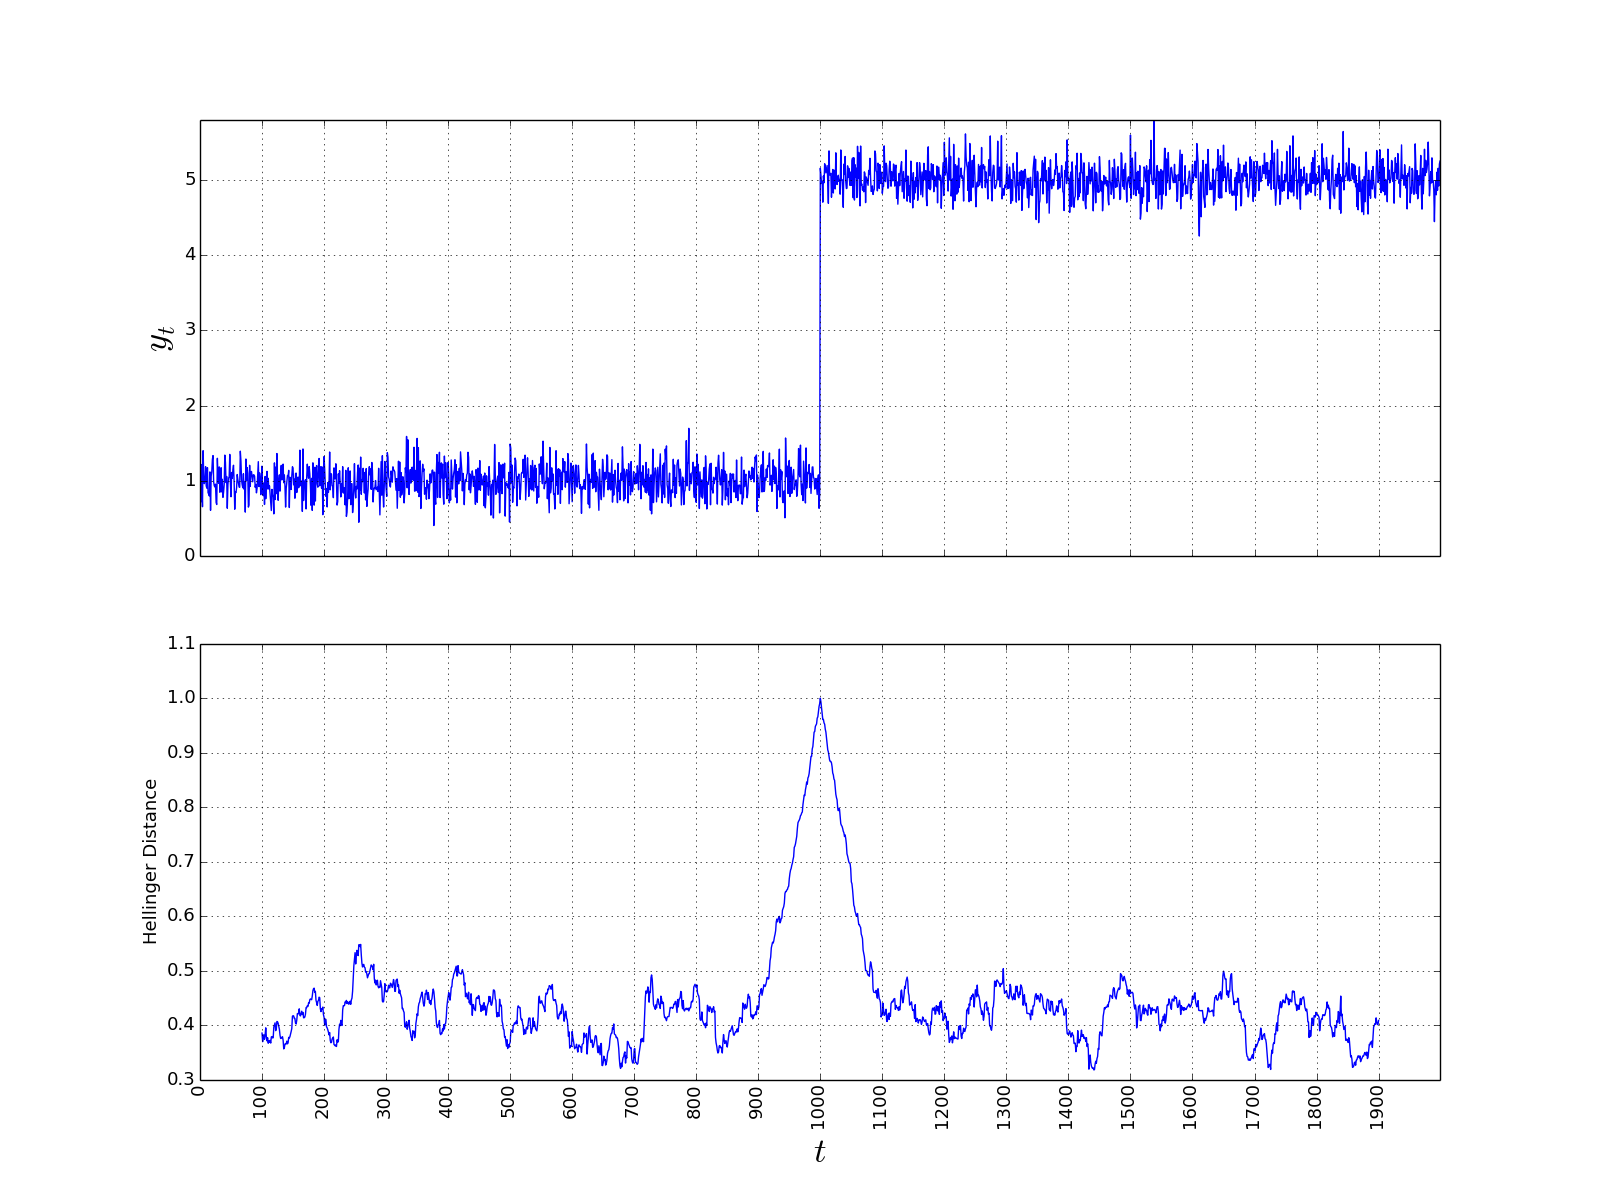
\includegraphics[width=1.0\textwidth]{./figures/sliding_window_toy_example.png}
    \caption{Toy example of a sliding windows method.}
    \label{fig:sliding_window_toy_example}
\end{figure}

It can be observed that there is a peak on the distance in the exact location where the distribution changed. However, using only the threshold method it is possible to prematurely infer the position of the change point, therefore, an alternative is to also use a peak detection algorithm. Besides, the distance function choice has a direct impact on the classification accuracy.

As stated in \cite{detecting_change_in_data_streams}, a performance improvement can be achieved concurrently executing the same sliding windows algorithm, however, with different windows lengths, which facilitates the detection of segments with distinct number of points.

\section{Optimization Model}  

Given a fixed value of $k$, one approach is to define a cost function that measures the homogeneity of a window, and therefore, choose the change points that globally optimize this homogeneity. Let the cost of the $i$-th segment be defined as $C(\mathbf{y}_{\tau_{i - 1} + 1 : \tau_{i}})$, then the cost of a segmentation is the sum of all segments costs.

A common choice for the function $C$ is the MSE (Mean Squared Error), which can capture changes in the mean. Another usual approach is to consider distribution changes through negative maximum log-likelihood functions, considering that data within a window is iid. 

Therefore, given a fixed $k$, the optimal segmentation is obtained through the following optimization problem, which is called the constrained case \cite{on_optimal_multiple_changepoint_algorithms_for_large_data}: 

\begin{equation}
    \min_{\boldsymbol \tau_{1 : k}} \sum \limits_{i = 1}^{k + 1} C(\mathbf{y}_{\tau_{i - 1} + 1 : \tau_{i}})
\end{equation}

This problem can be solved using dynamic programming with $O(k n^2 f(n))$ time complexity, where $f(n)$ is related with $C$ evaluation. Several segment cost functions can be evaluated in $O(1)$ after a $O(n)$ preprocessing phase, implying in an overall $O(k n^2)$ complexity. It is possible to proof that MSE, negative maximum log-likelihood functions of normal, exponential, poisson and binomial distributions have this characteristic. Also, the formulation can consider a minimum value of a window length.

Modeling segments with continuous distributions can lead to practical difficulties. One of them is the fact that segments can form degenerate distributions, that is, the data of a window can have zero variance, which is always the case of unitary length segments. In these scenarios the negative maximum log-likelihood is undefined. Two approaches can be used to overcome this situation. The first one tries to avoid degenerate segments adding a white noise with small variance to the time series. The second one considers that the cost of any degenerate distribution is equal to a constant.


% Using discrete distributions it is possible to easily compare direct compare the likelihood of two different distribution types. 

% Since the likelihood of different continuous distributions can`t be directly compared, is not possible to apply the segmentation algorithm considering different types of continuos distributions. One possibility to handle this is to apply automatic methods to check which kind of distribution fits better to the segment, such as Kolmogorov-Smirnov. This was not approached in this work due to the computation time efficiency decrease and that since we deal with small number of data possibly these methods would have a poor performance.

When the number of change points is unknown an usual way is to introduce a non decreasing penalty function $g(k)$. Then, the new optimization problem, called penalized case \cite{on_optimal_multiple_changepoint_algorithms_for_large_data}, is:

\begin{equation}
    \min_{k, \boldsymbol \tau_{1 : k}} \sum \limits_{i = 1}^{k + 1} C(\mathbf{y}_{\tau_{i - 1} + 1 : \tau_{i}}) + g(k)
\end{equation}

This problem can be solved in $O(K n^{2} f(n))$. However, if the penalty function is linear in $k$, the problem can be formulated more efficiently and solved in $O(n^{2} f(n))$.

Also, there are several pruning algorithms to speedup the computation \cite{optimal_detection_of_changepoints_with_a_linear_computational_cost, on_optimal_multiple_changepoint_algorithms_for_large_data, computationally_efficient_changepoint_detection_for_a_range_of_penalties}, in general trying to reduce the $\boldsymbol \tau$ search space but maintaining optimality.

\section{HMM (Hidden Markov Model)}

The idea that each segment is associated with a specific latent configuration has a direct interpretation to a HMM model \cite{a_hidden_markov_model_segmentation_procedure_for_hydrological_and_environmental_time_series, fast_estimation_of_posterior_probabilities_in_change-point_analysis_through_a_constrained_hidden_markov_model, inertial_hidden_markov_models_modeling_change_in_multivariate_time_series}. In this context, each window is related to a hidden state of a HMM, and the observation distribution of this state represents the distribution of that segment. Therefore, the mechanism models the time series using a HMM, and through the hidden state path assesses the times when a transition between different hidden states occur.

There are several approaches in the detection and training phases. For example, given a trained HMM, is possible to analyze the most probable hidden state path that a time series can follow through the viterbi algorithm. Also, it is possible to evaluate the probability of a transition between different hidden states at time $t$, and then apply a threshold and peak detection methods, as well as in sliding windows techniques. For the training step, it is possible to use several time series to train a single HMM, and then use this model to detect change points in all time series. Another way is to, for each time series, train a single model using only the target time series.

It is important to note that the structure of the hidden state graph has a large impact on the performance. Using a fully connected graph, the number of states defines the maximum number of distribution configurations. Employing a left to right structure, the number of hidden states will induce the maximum number of segments.

In \cite{inertial_hidden_markov_models_modeling_change_in_multivariate_time_series} is stated that when using a fully connected structure, the time interval that a time series stays in the same hidden state is low, which can not reflect real data. To overcome this problem, \cite{inertial_hidden_markov_models_modeling_change_in_multivariate_time_series} suggests to increase the time that a time series stands in the same hidden state, using a dirichlet prior regularization.

\section{Bayesian Inference}

There are several Bayesian methods with the objective to assess the probability that a point is a change point. Following an offline fashion, the work of \cite{exact_and_efficient_bayesian_inference_for_multiple_changepoint_problems} recursively calculates, for each $i$, the probability of $\mathbf{y}_{i : n}$ given a change point at $i$. With these probabilities is possible to simulate the time of the first change point, and then, compute the conditional distribution of the time of the second change given the first, and so on. To achieve this, the mechanism assumes that observations are independents, and that each segment is modeled by conjugate priors. Also, the procedure considers priors to model the number of changes and the time between two consecutive change points. The overall complexity of this method is $O(n^{2})$, considering that the likelihood of a segment can be evaluated in $O(1)$.

In \cite{bayesian_online_changepoint_detection} it is also considered that parameters of different segments are independents, and that data within a window is iid. However, through an online mode, the procedure is concerned with the estimation of the distribution of the length of the current time since the last change point, called run length, given the data so far observed. To achieve this, the method assumes the probability of current run length given the last run length as a prior. Assuming exponential-family likelihoods to model a segment, the time complexity to process a point is linear in the number of points already observed. 

    \chapter{Methodology}
\label{chap:methodology}

This chapter describes the proposed data analytics workflow.
Besides, the QoS data gathering procedures are briefly presented,
and the proposed system is compared with previous projects.

\section{Measurement Process}

The time series used in this work represent network end-to-end measures of a
cable-television infrastructure, which runs DOCSIS with asymmetric download and
upload bandwidths. A home router connected to a cable modem communicates
with a server strategically located by the ISP\@. Each server is responsible
for measurements of several end-users.
Measurements are triggered in
each home router every half hour and, by the end of every day,
the results are transferred to a database.
The software responsible for these procedures was
developed by TGR (a startup at UFRJ),
and is spread over approximately four thousand customers of a major Brazilian
Tier-3 ISP\@.

To measure the round
trip packet loss fraction and the RTT between the home router and the associated
server, the
home router sends a train of short UDP packets, and the server bounces back
them. The data here presented considers a train of 100 UDP packets of 32 bytes,
separated by 1 millisecond.
Maximum achievable upstream throughput is measured by overflowing the upload
links with parallel TCP data transfers from the end-user to the
server.
Also, the traceroutes from the end-users
to the respective servers are collected with the same frequency. Traceroutes
from servers to end-users are not gathered.
In~\cite{a_preliminary_performance_measurement_study_of_residential_broadband_services_in_brazil}
is presented a preliminary descriptive investigation of these metrics.

The resulted time series are unevenly spaced due to a range of reasons. First,
measurements are initiated only if the residential link is not under use by the
ISP customer. Also, the client may have no Internet connection to start a
measurement, or even be without electrical energy. Other details about the
measurement software are presented during the text, as they are needed.

\section{Pipeline}

This section describes, in a high level abstraction, the proposed workflow
used to detect network events and localize their cause. When necessary, some
steps are better explored in further sections.
The analysis seeks for events during a specific time period, in a single
measurement server, and considers an
particular metric (round trip, loss fraction, RTT, or maximum achievable
upstream throughput),
which are specified as parameters.
A complete analysis can be accomplished through different
executions with distinct parameters.
Figure~\ref{fig:pipeline} illustrates the process.

\begin{figure}[H]
    \centering
    \includegraphics[width=0.9\linewidth]{./figures/methodology/pipeline/pipeline.png}
    \caption{Pipeline.}
\label{fig:pipeline}
\end{figure}%

The workflow starts with the End-Users Filtering step,
which aims to remove clients that can negatively affect the analysis.
As an example, this work eliminates clients
with a small number of measurement samples.

The Change Point Detection phase preprocess the end-users time series and
identify change points.
Also, the change points are classified in three types of events: failure,
improvement, or inconclusive. For the used QoS metrics,
a change point defines a
failure event if the average of the window after this point is greater than the
average of the window before. The improvement event is analogous, however is
characterized by a mean decrease.
The inconclusive event means that the segments averages are too close.

The Spatial Correlation procedure clusterizes the end-users in user-groups
according with their position in the network. This clustering can then be used
in further steps to isolate possible events locations.
This stage must produce a specific grouping structure, which is detailed in
Section~\ref{sec:spatial_correlation}.

The Events Times Correlation aims to combine similar events of different
end-users. For example, if three end-users detect a failure at
the same time, then this information will be identified at this step.
The grouped end-users events of an user-group are named as network events.
The details of this method are enlightened in
Section~\ref{sec:events_times_correlation}.

Finally, to localize the events cause, the Spatial-Time Correlation method
matches network events with the user-groups structure.
This is better explained in Section~\ref{sec:spatial_time_correlation}.

\section{Spatial Correlation}
\label{sec:spatial_correlation}

This method provides the necessary information to check which network equipments
are shared by end-users that perceive the same network event.
The developed strategies were guided by the specific ISP's topology.

The server position relative to the end-user
can be categorized in two contexts.
In the OFF-NET case, the traffic between them
goes through a Tier-2 ISP\@.
In the ON-NET case, the traffic
doesn't leave the Tier-3 ISP infrastructure.
The latter situation represents a simpler IP topology, since the Tier-3 ISP
uses static routing and
doesn't applies load balancing nor MPLS, techniques that are usual in the Tier-2
ISP network.

Then, considering measurements against a single server and the ON-NET
case, paths from end-users to the server form a hierarchically
structured topology, which is a required design to be consumed by the
Spatial Time Correlation procedure~\ref{sec:spatial_time_correlation}.
This work doesn't have access to the ISP network
topology, therefore, this structure is reconstructed through traceroutes.
In this context, each equipment that responds to traceroute
pings is used as an user-group.
An user-group is formed by all end-users in which traceroutes contain the
associated network equipment.

The first hop of the traceroutes, which corresponds to the home gateway, is
removed from the analysis. Also, CMTSs are reported with their private IPs,
since they are in the same subnetwork of the end-users.
Therefore, to differentiate distinct CMTSs, the
user-groups are defined by their reported IP and the first public IP that
appears from their hop onward. Additionally, there are CMTSs
configured to not answer traceroute pings.

In the OFF-NET case, due to the load balancing applied by the Tier-2 ISP,
the traceroute reconstruction doesn't lead in a hierarchical topology.
Routers can implement three types of load balancing
policies~\cite{avoiding_traceroute_anomalies_with_paris_traceroute}.
The per
destination load balancing can be disconsidered in the current analysis, since
the target is always the same. The per flow load balancing attempts to
maintain packets from the same flow in the same path. A flow is identified
by header's fields of IP packets. For example, a
router can employ that packets with equal source/destination
address, protocol, and source/destination port,
belong to the same flow. The per packet load
balancing ensures that the load is equally distributed over the feasible output
links, deploying, for example, a round-robin strategy. However, the latter
method doesn't
make attempts to keep packets from the same flow in the same path.

For an end-user and server pair,
the measurement software uses the same ports over time to execute a specfic
measurement type, e.g., round trip loss fraction.
Hence, if routers only apply per flow load balancing,
and considering a time period without routing tables updates, and
depending of which IP header's fields are used to define a flow, it is possible
that all packets generated by a specific measurement type traverse the same
path. However, these are strong and unlikely suppositions.
Additionaly, since the implemented traceroute also uses the same ports over
time, and considering that different measurements types use distinct ports,
the
path followed by traceroute packets can be different from the path folowed by
the QoS mesurements packets. Then, in this scenario, even with static paths in
the Tier-2 ISP network, the correlation between traceroutes
results with end-to-end metrics can reach wrong conclusions.

Therefore, this work supposes that the Tier-2 ISP only applies per packet load
balancing, which is modeled here as a random strategy. With this hypothesis,
if two end-users are geographically near, then it is likely that their packets
traverse in the same set of routers in the Tier-2 network. This implies that if
an event occur in a Tier-2 router, it is not possible that only one of these
end-users perceive the event. This is a important consequence explored in
Section~\ref{sec:spatial_time_correlation}.

To handle the OFF-NET case, sequential hops related to
the Tier-2 ISP are compressed to a single hop.
As an example, the path (Tier-3 Router 1, Tier-2 Router 1, Tier-2 Router 2,
Tier-3 Router 2, Server) is
transformed to (Tier-3 Router 1, Tier-2, Tier-3 Router 2, Server).
In general, this process conducts to a hierarchical topology.
The exception occurs when the Tier-2 ISP has output connections to
different routers of the Tier-3 ISP in the same network region.
However, this is an unusual situation in
the current dataset, and therefore, was removed from the analysis.
The distinction between
Tier-3 and Tier-2 hops is made through the investigation of hop names.

Figure~\ref{fig:real_graph} presents an example of the reconstructed
topology. The equipments were anonymised. The ``Tier-2'' and ``Server''
user-groups are self explanatory. The others are represented by a tuple, in
which the first field indicates the reported IP in the traceroute, and the
second specifies the first hop, from the associated position onward,
that reported a public IP\@.

\begin{figure}[H]
    \centering
    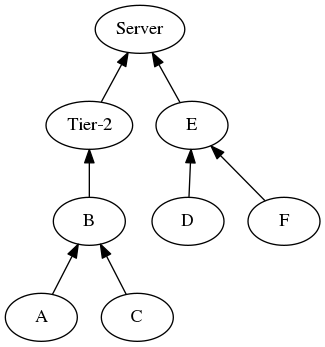
\includegraphics[width=\linewidth]{./figures/methodology/spatial_correlation/dtstart2016-05-01_dtend2016-05-11_NRIDTCLDM031_graph_anonymized.png}
    \caption{User-groups structure.}
\label{fig:real_graph}
\end{figure}%

Since the links were oriented from the end-users to the server,
it is possible to model this structure as a DAG\@. The zero
in degree vertexes indicate equipments that only appear as the first hop,
however, an internal vertex can be a first hop in a traceroute.
Considering an arc (A, B), all users who belong to A also belong to B,
but the inverse is not necessarily true.

During the End-Users Filtering step, some clients are removed due to traceroute
inconsistencies~\cite{avoiding_traceroute_anomalies_with_paris_traceroute}.
As an example, there are cases in which the same equipment appears in different
hops of the same end-user traceroute. Also,
the measurement software limits the maximum number of hops, then,
scenarios in which the traceroute doesn't reach the server are discarded.
Since routing tables can be updated, after the Tier-2 vertexes compression,
it is only considered clients with static traceroutes
during the specified time period.
Situations characterized by Tier-2 routers that doesn't appear as consecutive
elements in the traceroute are also deleted.

\section{Events Times Correlation}
\label{sec:events_times_correlation}

The motivation of this mechanism is to infer network events that can explain
end-users events of an user-group.

There are two main reasons to detect the same network event, such as an
equipment failure, at different times in different clients. The first one is
related to the fact that the time series are not regularly sampled. The second
one is due to the change point detection algorithm behavior.
Therefore, a procedure to group end-users events based on their type and time,
should be flexible enough to take into consideration time delay effects. Also,
it must be robust to deal with multiple change points per time series.

In order to relax a change point location, a detected change point is
transformed into an interval according to a time tolerance.
Therefore, given a parameter $\delta$, a change point identified at
time $t$ implies in the existence of a change point within
$[t - \delta, t + \delta]$. To be consistent,
change point algorithms must report locations separated by more than
$2 \delta$ time units. In general, the algorithms presented in
Chapter~\ref{chap:change_point_detection}
can be adapted to respect this restriction. However, this can also be
achieved by the following post processing step:
sweeping time from left to right, if two
points are at most $2 \delta$ time units apart, then the right one is removed.

Consequently, the problem can be defined as selecting a set of network events,
that explain all end-users events. It is important to note that events are
defined only by their time and type.
An end-user event is explained by a network event if they have the same type,
and the end-user event time is inside the network event time interval.
This problem has several possible solutions, and the comparison between
them is subjective. As an example, not
necessarily selecting the minimum number of network events that cover all
end-user events is the most appropriate answer.

To this goal, it was developed a heuristic inspired in the Inexact Voting in
Totally
Ordered Space problem~\cite{voting_algorithms}. In this problem, people
vote in a single point in the real line. Also considering a $\delta$
parameter, the objective is to
select the interval with the greatest number of voters.

The created greedy procedure, called here as Multiple Inexact Voting in Totally
Ordered Space, is specified in
Algorithm~\ref{alg:multiple_inexact_voting_totally_ordered_space}

\begin{algorithm}[H]
\caption{Multiple Inexact Voting in Totally Ordered Space}
\label{alg:multiple_inexact_voting_totally_ordered_space}
    \begin{algorithmic}[1]
        \State{Let $l$ be the end-users events of a specific type sorted by
        time}
        \While{$l$ is not empty}
            \State{Select the interval $d$ with the greatest number of
            end-users events,
            in which all these events are at most $2 \delta$ apart.
            In case of ties, select the left most one}
            \State{Report the mean time of
            the $d$ extremes as the network event time}
            \State{Remove all end-users events from $l$ that are in $d$}
        \EndWhile{}
    \end{algorithmic}
\end{algorithm}

It is possible to note that, in each iteration the procedure solves an instance
of the Inexact Voting in Totally Ordered Space.
The proposed algorithm is executed three times in every user-group,
one for each event type.

A more straighforward solution, that was not used in this work, is to create
regular time-bins, and interpret all end-users events that occur at the same
bin as a common network event.
However, this strategy can introduce
discontinuities. If a network event occurs in the end/beginning of a time-bin,
then it is likely to different end-user events, associated with this
network event, be located in different bins.

If co-occurrent events with the same type affect the same end-users set,
it is not possible to distinguish them. Nonetheless, the chances of
detecting different events at the same time can reduce with the increase
of the time series sampling frequency.

\section{Spatial-Time Correlation}
\label{sec:spatial_time_correlation}

This step matches network events from different user-groups to define
a set of feasible events locations.

It is not possible to check if changes in round trip metrics, such as RTT,
are caused in the path from the end-user to the server or vice versa.
Therefore, correlate those metrics with the available traceroutes can lead to
erroneous or inconclusive outcomes. Also, the maximum achievable upstream
throughput can be affected by a service degradation on the path from the server
to the end-user, since losses of TCP's ACKs can influence the measurement
performance.
Hence, this work restricts to report possible events locations considering that
they are caused by equipments in the path from the end-user to the server.

The method expects that
a change point detection algorithm setup is able to detect all end-users
affected by a network event, or no end-user is identified.
Besides, with exception of the Tier-2 user-group, the mechanism supposes that
if an event occur in an user-group,
all traffic that goes through this cluster is affected by the event. Since
there is a direct connection between an user-group and an unique network
equipment, this is a reasonable hypothesis.

In the first reasoning part, it will be processed cases without the
presence of the Tier-2 user-group. Also, it will be removed
traceroutes paths that doesn't start in a zero indegree vertex.
Additionally, it will be disconsidered co-occurrent events with the same type.
Later, these restrictions will be removed and treated separately.
Unless stated differently, in the rest of this section is considered an
unique network event in the period of study.

The procedure starts analysing zero indegree vertexes.
Suppose that only a proper subset of the clients that belong to a zero
indegree node perceive the event. In this situation, it is possible to afirm
that this vertex is not the cause of the event, since not all clients detected
it. For the same reason, the cause is not located in posterior nodes
in the path to server.
Then, if this set size is bigger than one, these end-users must share
a network equipment, which is the cause, that doesn't respond to traceroute
pings, and is located before the first hop. As an example,
this equipment can be a fiber node.

However, if all clients of the zero indegree vertex detect the event, then
there are three options:
this vertex can be the cause, or these end-users can share an equipment before
the first hop that explains the event,
or the cause is located after the first hop. Due to the
lack of information about the topology above the IP layer, the first two cases
can't be
distinguished. Nonetheless, to check the latter scenario, the same type of
analysis is applied to the next vertex in the path to the server. If not all
clients of the second hop detected this event, then the event is surely located
in the first hop or before. Otherwise, the procedure continues to the next hop.

When applied to different zero indegree vertexes,
this method results in possible events locations that are prefixes of
the paths to the server.
However, different paths share common network equipments, then these prefixes
can be correlated.

If different paths detect the same network
event, then they must share at least one equipment. The
ones that are not common can be discarded from the possible cause list, since
there are end-users that dont't belong to them and still perceive the event.

Figure~\ref{fig:network_events_locations_examples} presents several topologies
and different network events. The gray vertexes indicate a network event
that occurred in this location.

\begin{figure}[H]
    \centering
    \makebox[\textwidth][c]{%
        \begin{subfigure}[b]{0.2\textwidth}
            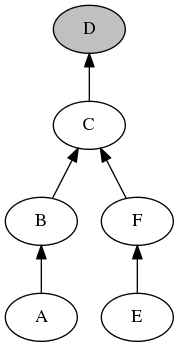
\includegraphics[width=\textwidth]{./figures/methodology/spatial_time_correlation/event_tree_graph_1.png}
            \caption{}\label{fig:network_events_locations_examples_1}
        \end{subfigure}
        \begin{subfigure}[b]{0.2\textwidth}
            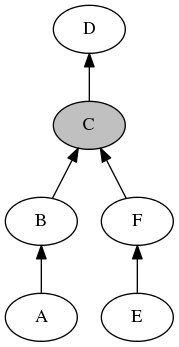
\includegraphics[width=\textwidth]{./figures/methodology/spatial_time_correlation/event_tree_graph_2.png}
            \caption{}\label{fig:network_events_locations_examples_2}
        \end{subfigure}%
        \begin{subfigure}[b]{0.3\textwidth}
            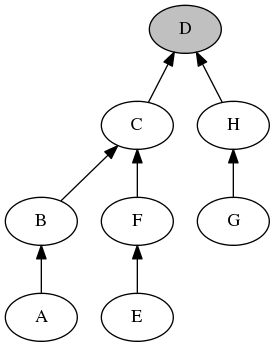
\includegraphics[width=\textwidth]{./figures/methodology/spatial_time_correlation/event_tree_graph_3.png}
            \caption{}\label{fig:network_events_locations_examples_3}
        \end{subfigure}
        \begin{subfigure}[b]{0.3\textwidth}
            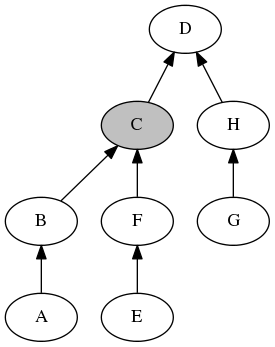
\includegraphics[width=\textwidth]{./figures/methodology/spatial_time_correlation/event_tree_graph_4.png}
            \caption{}\label{fig:network_events_locations_examples_4}
        \end{subfigure}%
    }
    \caption{Network event location examples.}
\label{fig:network_events_locations_examples}
\end{figure}%

In Figure~\ref{fig:network_events_locations_examples_1}, the analysis
starting at vertex A results in the following feasible event locations,
\{A, B, C, D\}. The reasoning through node E leads to
\{E, F, C, D\}. Correlating both results, the possible locations are \{C, D\}.
Figure~\ref{fig:network_events_locations_examples_2} presents a scenario with
the same conclusion.

In Figure~\ref{fig:network_events_locations_examples_3}, the analyis made
through the zero indegree vertexes result in the paths from them to the server.
Matching the outcomes, the D vertex is the only possible event location.

In Figure~\ref{fig:network_events_locations_examples_4}, the reasoning through
node G doesn't detect the event. The analysis in A finds \{A, B, C\}. Through
node E, \{E, F, C\} is the result.
Correlating the outcomes, C is the only feasible event location.

The previous analysis can't be fully applied in situations with the Tier-2
user-group.
As an example, suppose two geographically distant end-users in an OFF-NET case.
The packets from these two users can go through completely different paths in
the Tier-2 ISP\@. Then, it is possible that an event in the Tier-2 ISP only
affects one of the users, which contradicts one of the established restrictions.
To overcome this issue, when analysing a path, if an event can be located in the
previous hop of the Tier-2 user-group, then the event can also be located at
the Tier-2 vertex, even considering that not all end-users of this user-group
perceived the event.

Now, suppose paths that doesn't start in zero indegree vertexes, which should
be processed after the analysis explained above.
If all clients of the first hop user-group detect the event, then this
path was already treated. Otherwise, the end-users that detected the event
share an equipment, that doesn't answer to traceroute pings and is the cause.

If there are co-occurrent events with the same type, the complete procedure can
result in a wrong outcome. Figure~\ref{fig:network_events_locations_examples_5}
illustrates this case.

\begin{figure}[H]
    \centering
    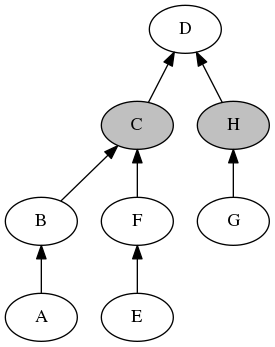
\includegraphics[width=0.35\linewidth]{./figures/methodology/spatial_time_correlation/event_tree_graph_5.png}
    \caption{Co-occurent events.}
\label{fig:network_events_locations_examples_5}
\end{figure}%

Through node A, the feasible locations are \{A, B, C, D\}.
Checking E, the result is \{E, F, C, D\}.
In vertex G, the outcome is \{G, H, D\}.
Correlating the paths results leads to the location D, which is a mistake.
Therefore, when considering co-occurrent events with the same type, the step of
correlating the conclusions of different paths must not be applied, and the
union of these results should be the final outcome.

From this procedure, it is possible to formulate a
problem to define the minimum number of end-users to be monitored, and their
placement to localize events with the minimum number of feasible locations.

\section{Change Point Detection Issues}

As stated in Chapter~\ref{chap:change_point_detection}, one of the main issues
of this work is the algorithms and parameters selection.
In general, this process requires a dataset to enable the evaluation of an
algorithm setup.

There are several approaches to construct a
change points dataset in the literature.
Some works create simulated time series, in which distinct segments are sampled
by the same generative model with different
parameters~\cite{change_point_detection_in_time_series_data_by_relative_density_ratio_estimation}.
In general, this type of data is more easily handled by change point detection
algorithms, since some methods assume the same models used in the dataset
building process. Also, real data can have complex characteristics that are
difficult to be reproduced by generative models. Another strategy is to join
segments from different real time series with different
characteristics~\cite{inertial_hidden_markov_models_modeling_change_in_multivariate_time_series}.
However, this can introduce unreal change points scenarios. Since one of
the goals of this work is to deal directly with real data,
this approach was discarded.

When the latent information of the time series are available, and if there is a
complete knowledge of what configurations changes in the latent state impact
data, it is possible to check the change points only analyzing this underlying
information. As an example, consider a time series that represents the cardiac
frequency of a soccer player during a match. Also, consider that in this
controlled environment, the only causes of changes in the cardiac frequency are
the variations of physical activities, such as starting or stopping to run.
Therefore,
it is possible to use the times in which a player changed his movement behavior
as the change points, whithout even analyzing the time series. However, in the
application domain of the present work, this approach would be impractical.
First, this would need the expertise of how the configurations of network
topology, routers congestion, physical equipment problems, among other features,
affect the different end-to-end QoS metrics.
Second, this kind of information is absent in the dataset, and would be too
complex to collect it.

Another way is to use visual annotations,
as it was done
in~\cite{learning_sparse_penalties_for_change_point_detection_using_max_margin_interval_regression}.
Also, manual labeling is usual for anomaly indentification in Interner traffic
traces~\cite{webclass_adding_rigor_to_manual_labeling_of_traffic_anomalies}.
In this strategy, an application domain expert is exposed to a time series,
and visually indicates his opinion about the change points locations.

It is known that visual inspection methods can bring erroneous
conclusions~\cite{leveraging_cloud_data_to_mitigate_user_experience_from_breaking_bad},
and also amplify subjectivity, however, to better understand the problem, this
approach was experimented in this work.

Through a web system a user freely marked the change points with a mouse.
The fact that data is not regularly sampled in time could bring an unwanted
visual change perception. Therefore, the X axis of the displayed time series
represented only the temporal order of the measures.
It was only presented raw
loss fraction time series with 10 days of data.
Also, it was selected the ones that have at
least 85\% of the maximum possible number of points during the specified period,
considering that data is sampled at most two times in a hour. Change points can
be interpreted as rare events in this dataset, and several data streams have
almost
all measures with zero losses. Therefore, to increase the entropy,
it was selected time series that have at least one window of length 48 with
more than 5 measures with loss fraction larger than 0.01.

Additionally, it was provided a set of tips to the specialist:

\begin{itemize}
    \item In the case of packet loss fraction, mean changes between 0 and 0.1
    are more sensible to the end users.
    \item The time axis only represents the temporal order of the measurements.
    However, in general, consecutive points in time axis are separated by 30
    minutes.
    \item Outlier is not a statistical change. An outlier is an observation that
    lies outside the overall pattern of a distribution.
\end{itemize}

Figure~\ref{fig:survey_system} presents a system snapshot.
The vertical red line means that the user marked a change point in that
position.

\begin{figure}[H]
    \centering
    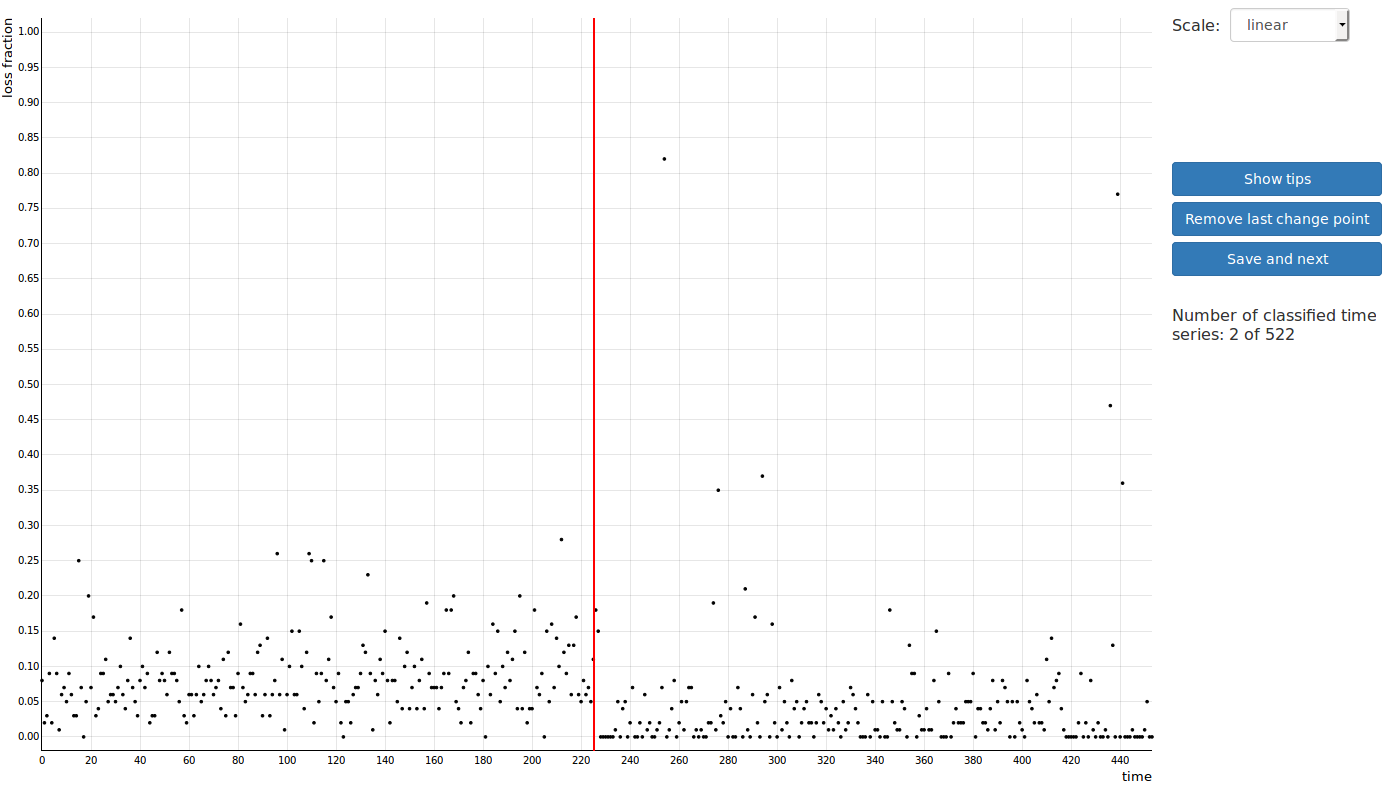
\includegraphics[width=0.9\linewidth]{./figures/methodology/supervised_learning_try/survey_system.png}
    \caption{Survey system snapshot.}
\label{fig:survey_system}
\end{figure}%

Six specialists with experience in network measurements and statistical
modeling, but without background in change point detection, classified 71 time
series.
To analyze the agreement between different users classifications,
for each time series, was applied the Events Times Correlation
procedure~\ref{sec:events_times_correlation}. Therefore, it was
considered that each specialist voted to a set of change points positions.
The time tolerance was set to 7 hours, which means 14 consecutive points.

Then, for each change point voted at least once, it was counted the number of
specialists that voted in that location.
Figure~\ref{fig:classifications_per_vote} shows the histogram of this counting.

\begin{figure}[H]
    \centering
    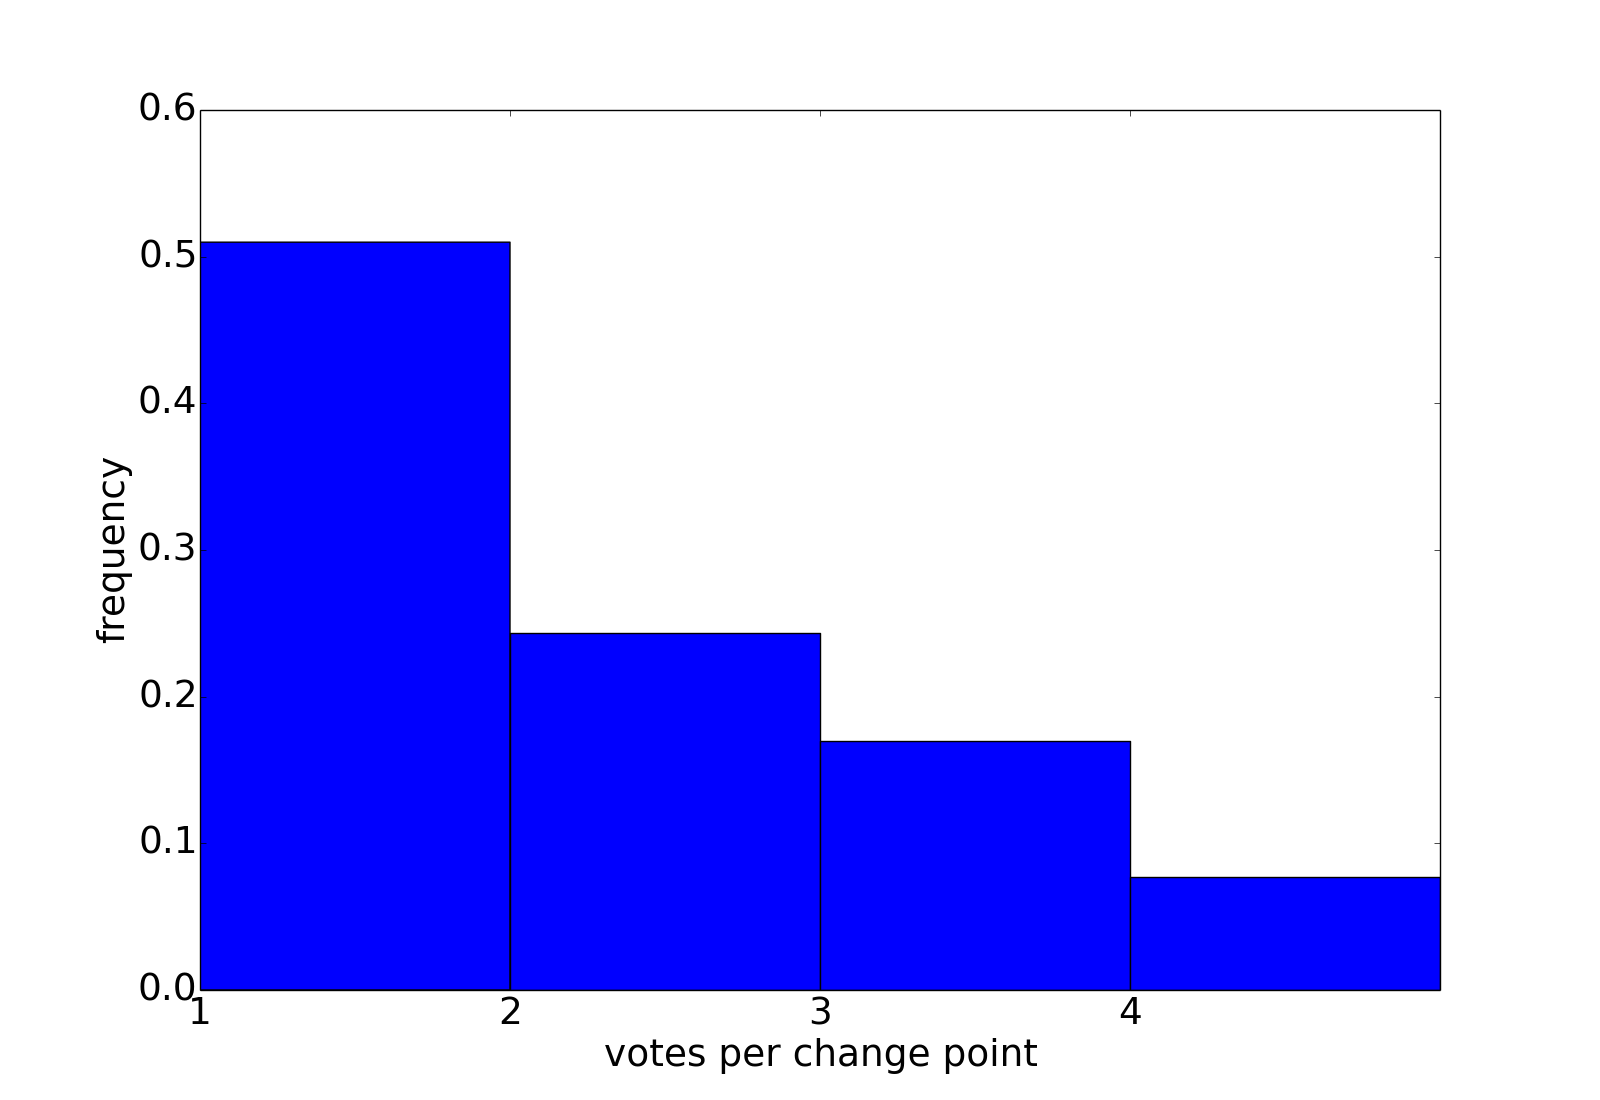
\includegraphics[width=0.7\linewidth]{./figures/methodology/supervised_learning_try/cnt_classifications_per_vote.png}
    \caption{Number of votes per change point histogram.}
\label{fig:classifications_per_vote}
\end{figure}%

It is possible to note that, 44\% of the change points were only voted by
a single user, and only 23\% were voted by the majority (more than 3 votes).
Therefore, in general, the consensus of change point locations is low.

In Figure~\ref{fig:classification_match} is presented the specialists
classifications in a time series with a high level of agreement on the change
points locations.

\begin{figure}[H]
    \centering
    \makebox[\textwidth][c]{%
        \begin{subfigure}[b]{0.55\textwidth}
            \includegraphics[width=\textwidth]{{./figures/methodology/supervised_learning_try/cnt6_serverNHODTCSRV04_mac64:66:B3:A6:BC:B8_dtstart2016-05-01_dtend2016-05-11/rosam@land.ufrj.br}.png}
            \caption{Specialist 1}\label{fig:classification_match_1}
        \end{subfigure}
        \begin{subfigure}[b]{0.55\textwidth}
            \includegraphics[width=\textwidth]{{./figures/methodology/supervised_learning_try/cnt6_serverNHODTCSRV04_mac64:66:B3:A6:BC:B8_dtstart2016-05-01_dtend2016-05-11/gustavo.santos@tgr.net.br}.png}
            \caption{Specialist 2}\label{fig:classification_match_2}
        \end{subfigure}
    }
    \makebox[\textwidth][c]{%
        \begin{subfigure}[b]{0.55\textwidth}
            \includegraphics[width=\textwidth]{{./figures/methodology/supervised_learning_try/cnt6_serverNHODTCSRV04_mac64:66:B3:A6:BC:B8_dtstart2016-05-01_dtend2016-05-11/guisenges@land.ufrj.br}.png}
            \caption{Specialist 3}\label{fig:classification_match_3}
        \end{subfigure}
        \begin{subfigure}[b]{0.55\textwidth}
            \includegraphics[width=\textwidth]{{./figures/methodology/supervised_learning_try/cnt6_serverNHODTCSRV04_mac64:66:B3:A6:BC:B8_dtstart2016-05-01_dtend2016-05-11/gabriel.mendonca@tgr.net.br}.png}
            \caption{Specialist 4}\label{fig:classification_match_4}
        \end{subfigure}
    }
    \makebox[\textwidth][c]{%
        \begin{subfigure}[b]{0.55\textwidth}
            \includegraphics[width=\textwidth]{{./figures/methodology/supervised_learning_try/cnt6_serverNHODTCSRV04_mac64:66:B3:A6:BC:B8_dtstart2016-05-01_dtend2016-05-11/edmundosilva@gmail.com}.png}
            \caption{Specialist 5}\label{fig:classification_match_5}
        \end{subfigure}
        \begin{subfigure}[b]{0.55\textwidth}
            \includegraphics[width=\textwidth]{{./figures/methodology/supervised_learning_try/cnt6_serverNHODTCSRV04_mac64:66:B3:A6:BC:B8_dtstart2016-05-01_dtend2016-05-11/edmundo@land.ufrj.br}.png}
            \caption{Specialist 6}\label{fig:classification_match_6}
        \end{subfigure}
    }
    \caption{Classifications agreements.}
\label{fig:classification_match}
\end{figure}%

Figure~\ref{fig:classification_mismatch} shows a time series with
several disagreements.
It was verified that this case is the most representative in the
constructed dataset, fact that corroborates with the problem subjectiveness.

\begin{figure}[H]
    \centering
    \makebox[\textwidth][c]{%
        \begin{subfigure}[b]{0.55\textwidth}
            \includegraphics[width=\textwidth]{{./figures/methodology/supervised_learning_try/cnt6_serverCTBDTCLDM91_mac64:66:B3:A6:B7:BC_dtstart2016-05-01_dtend2016-05-11/rosam@land.ufrj.br}.png}
            \caption{Specialist 1}\label{fig:classification_mismatch_1}
        \end{subfigure}
        \begin{subfigure}[b]{0.55\textwidth}
            \includegraphics[width=\textwidth]{{./figures/methodology/supervised_learning_try/cnt6_serverCTBDTCLDM91_mac64:66:B3:A6:B7:BC_dtstart2016-05-01_dtend2016-05-11/gustavo.santos@tgr.net.br}.png}
            \caption{Specialist 2}\label{fig:classification_mismatch_2}
        \end{subfigure}
    }
    \makebox[\textwidth][c]{%
        \begin{subfigure}[b]{0.55\textwidth}
            \includegraphics[width=\textwidth]{{./figures/methodology/supervised_learning_try/cnt6_serverCTBDTCLDM91_mac64:66:B3:A6:B7:BC_dtstart2016-05-01_dtend2016-05-11/guisenges@land.ufrj.br}.png}
            \caption{Specialist 3}\label{fig:classification_mismatch_3}
        \end{subfigure}
        \begin{subfigure}[b]{0.55\textwidth}
            \includegraphics[width=\textwidth]{{./figures/methodology/supervised_learning_try/cnt6_serverCTBDTCLDM91_mac64:66:B3:A6:B7:BC_dtstart2016-05-01_dtend2016-05-11/gabriel.mendonca@tgr.net.br}.png}
            \caption{Specialist 4}\label{fig:classification_mismatch_4}
        \end{subfigure}
    }
    \makebox[\textwidth][c]{%
        \begin{subfigure}[b]{0.55\textwidth}
            \includegraphics[width=\textwidth]{{./figures/methodology/supervised_learning_try/cnt6_serverCTBDTCLDM91_mac64:66:B3:A6:B7:BC_dtstart2016-05-01_dtend2016-05-11/edmundosilva@gmail.com}.png}
            \caption{Specialist 5}\label{fig:classification_mismatch_5}
        \end{subfigure}
        \begin{subfigure}[b]{0.55\textwidth}
            \includegraphics[width=\textwidth]{{./figures/methodology/supervised_learning_try/cnt6_serverCTBDTCLDM91_mac64:66:B3:A6:B7:BC_dtstart2016-05-01_dtend2016-05-11/edmundo@land.ufrj.br}.png}
            \caption{Specialist 6}\label{fig:classification_mismatch_6}
        \end{subfigure}
    }
    \caption{Classifications disagreements.}
\label{fig:classification_mismatch}
\end{figure}%

Also, it is possible to note that some users apparently changed their
classification pattern in the same time series. As an example,
Figure~\ref{fig:diff_class_same_time_series} presents two specialists that fits
this description. Also, in general, users changed their classification pattern
in different time series.

\begin{figure}[H]
    \centering
    \makebox[\textwidth][c]{%
        \begin{subfigure}[b]{0.55\textwidth}
            \includegraphics[width=\textwidth]{{./figures/methodology/supervised_learning_try/cnt6_serverNHODTCSRV04_mac64:66:B3:A6:B6:36_dtstart2016-05-01_dtend2016-05-11/rosam@land.ufrj.br}.png}
            \caption{Specialist 1}\label{fig:diff_class_same_time_series_1}
        \end{subfigure}
        \begin{subfigure}[b]{0.55\textwidth}
            \includegraphics[width=\textwidth]{{./figures/methodology/supervised_learning_try/cnt6_serverNHODTCSRV04_mac64:66:B3:A6:B6:36_dtstart2016-05-01_dtend2016-05-11/edmundo@land.ufrj.br}.png}
            \caption{Specialist 6}\label{fig:diff_class_same_time_series_6}
        \end{subfigure}
    }
    \caption{Different classification pattern in the same time series.}
\label{fig:diff_class_same_time_series}
\end{figure}%

Since this initial experiment resulted in a noisy dataset, in which change
points probably don't reflect real network events, this strategy was aborted.
Also, it would be difficult to scale the study to include more
specialists and time series.

It is important to note that the algorithms described in
Chapter~\ref{chap:change_point_detection} are unsupervised methods.
Once a change point dataset is constructed, it is possible to apply supervised
learning procedures, which are not much explored in the change
point detection literature.

\section{Differences to Previous Systems}

The proposed data analytics architecture has several similarities with the
projects described in Chapter~\ref{chap:literature_review}.

As with Argus and NetNorad, this work clusters end-users in user-groups, however
with finer topology granularity. Also, to increase the system's scalability,
NetNorad and Argus use this grouping to reduce the number of tracked time
series. This strategy was not applied in this project,
since the finer granularity requires more time series to be spread in different
network locations, and the current dataset has a low number of end-users.

To detect faults, Argus applies an anomaly detection procedure, but the present
work uses a change point detection method. The difference between
these two problems is subtle, and can be fuzzy in the literature. The
anomaly detection assumes that a standard pattern is already known or
is identified by the procedure, then the goal is to find when the data
stream
deviates from it's standard. The change point detection only seeks for
points where the statistical properties change, and doesn't take into
consideration a standard time series behaviour.

Additionally, beyond the network edge point of view, Argus and NetNorad
uses some internal network information, which is absent in the present work.

    \chapter{Results}
\label{chap:results}

As stated in Chapter~\ref{chap:methodology}, due to the absence of an events
dataset, it is not possible to extensively study the system's accuracy.
However, this chapter presents illustrative examples when the proposed pipeline
was applied to real data.

It was considered 7 months of measurements, from may to November 2016.
This data was then split in batches of 10 days, and for each batch,
a complete offline analysis was executed.
Considering the 35 servers, the mean number of client-server
pairs, in which occurred at least one measurement between them during a batch,
was 2246.
After the End-Users Filtering step, this average reduced to 741.
In general, one client measured against a single server through the batch.

For all cases, the time series were preprocessed with a median filter.
The change points were detected through the optimization model described in
Chapter~\ref{chap:change_point_detection}.
For each \gls*{qos} metric, the algorithms' hyperparameters were manually selected.
It was opted by conservative values, in order to avoid change points that,
through a visual inspection, may be arguably not related to a network event.
These algorithms choices were guided by two facts.
First, through a empirical visual analysis,
it was verified their reasonable performance with real data.
Also, the impact of their hyperparameters can be easily interpreted, which is
an important feature for manual tuning.

The fraction of clients threshold, used to check if an event can be
located in a vertex, was set to 0.75. The $\delta$ parameter, used to verify if
two change points are near, was set to 8 hours.

Section~\ref{sec:possible_correct_outcomes} presents examples with potential
correct outcomes, and Section~\ref{sec:possible_wrong_outcomes} exposes
cases with possible wrong results. These conclusions were manually corroborated
with a visual check.

\section{Possible Correct Outcomes}
\label{sec:possible_correct_outcomes}

Figure~\ref{fig:before_first_hop} shows a proper subset of clients that belong
to a specific user-group modeled by a zero indegree vertex.

\begin{figure}[H]
    \centering
    \makebox[\textwidth][c]{%
        \begin{subfigure}[b]{0.55\textwidth}
            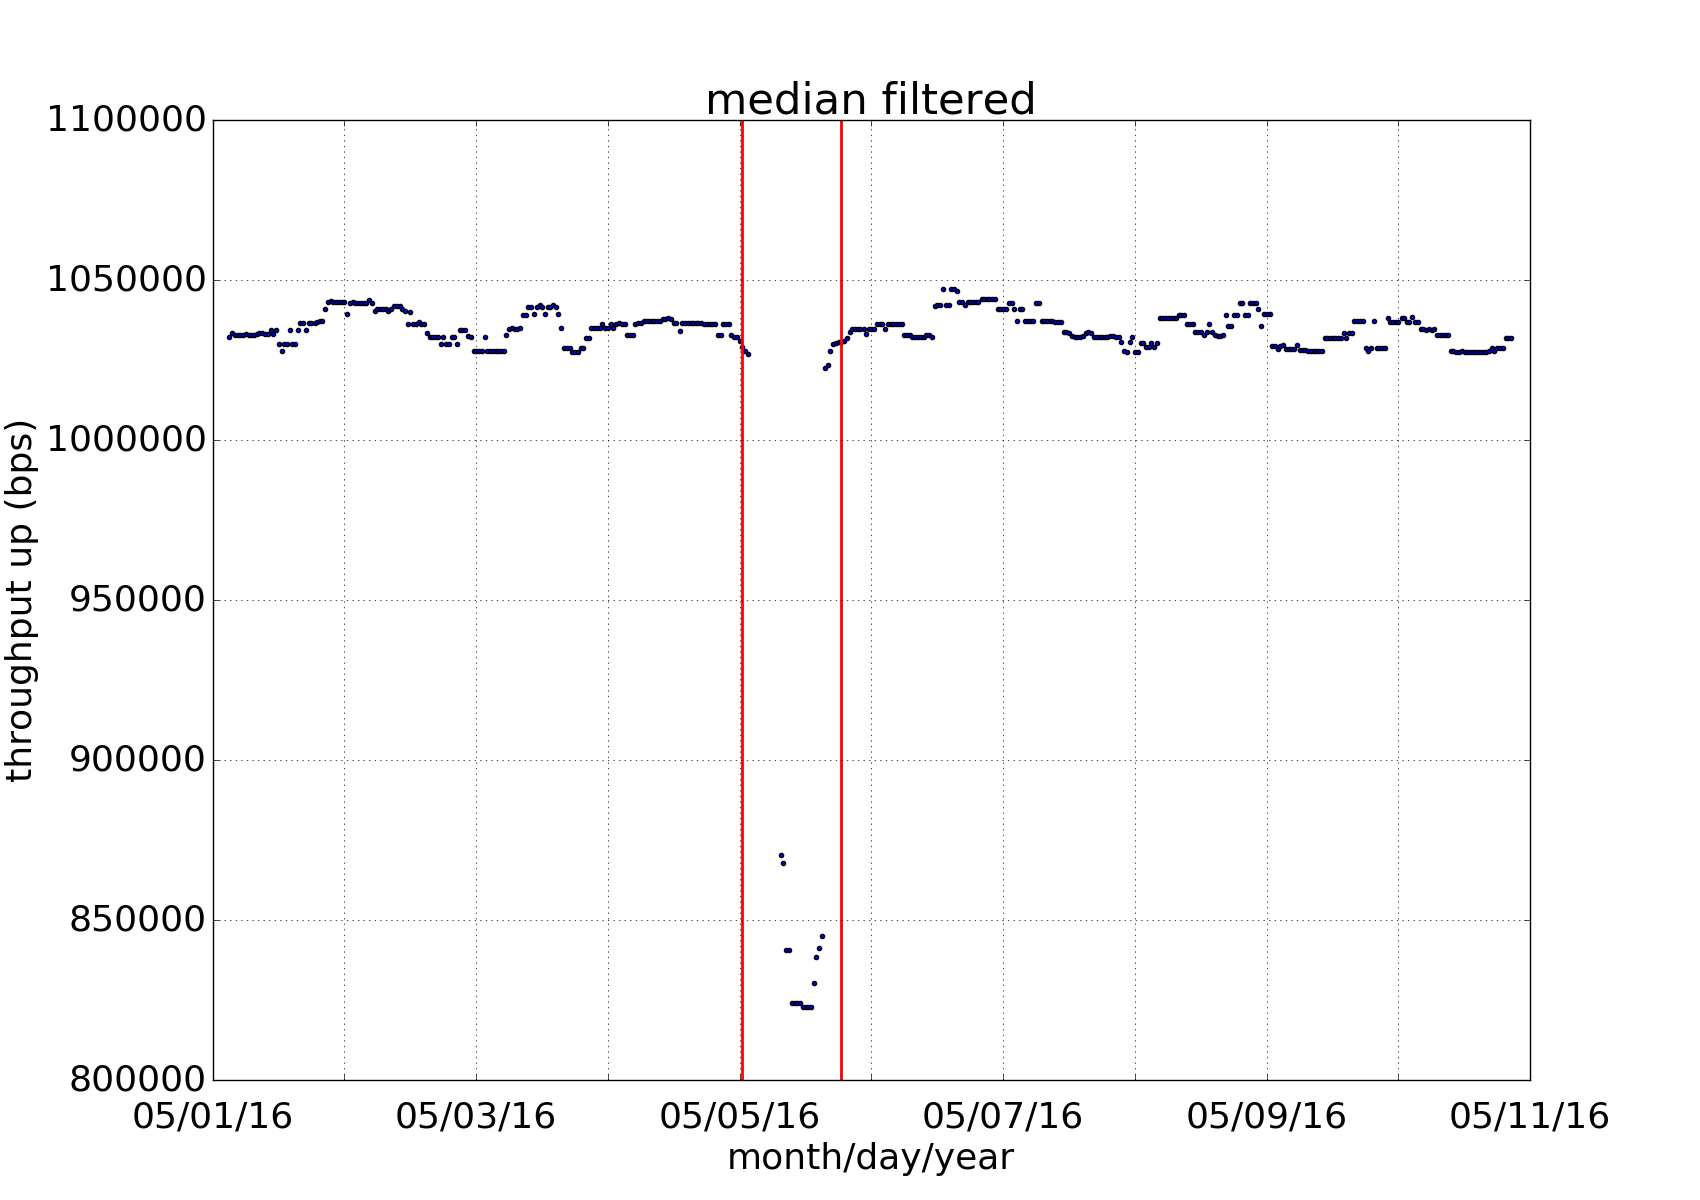
\includegraphics[width=\textwidth]{./figures/results/correct_examples/before_first_hop/serverSDRDTCLDM012_mac64:66:B3:50:06:D4_dtstart2016-05-01_dtend2016-05-11.png}
            \caption{Client 1.}
        \end{subfigure}
        \begin{subfigure}[b]{0.55\textwidth}
            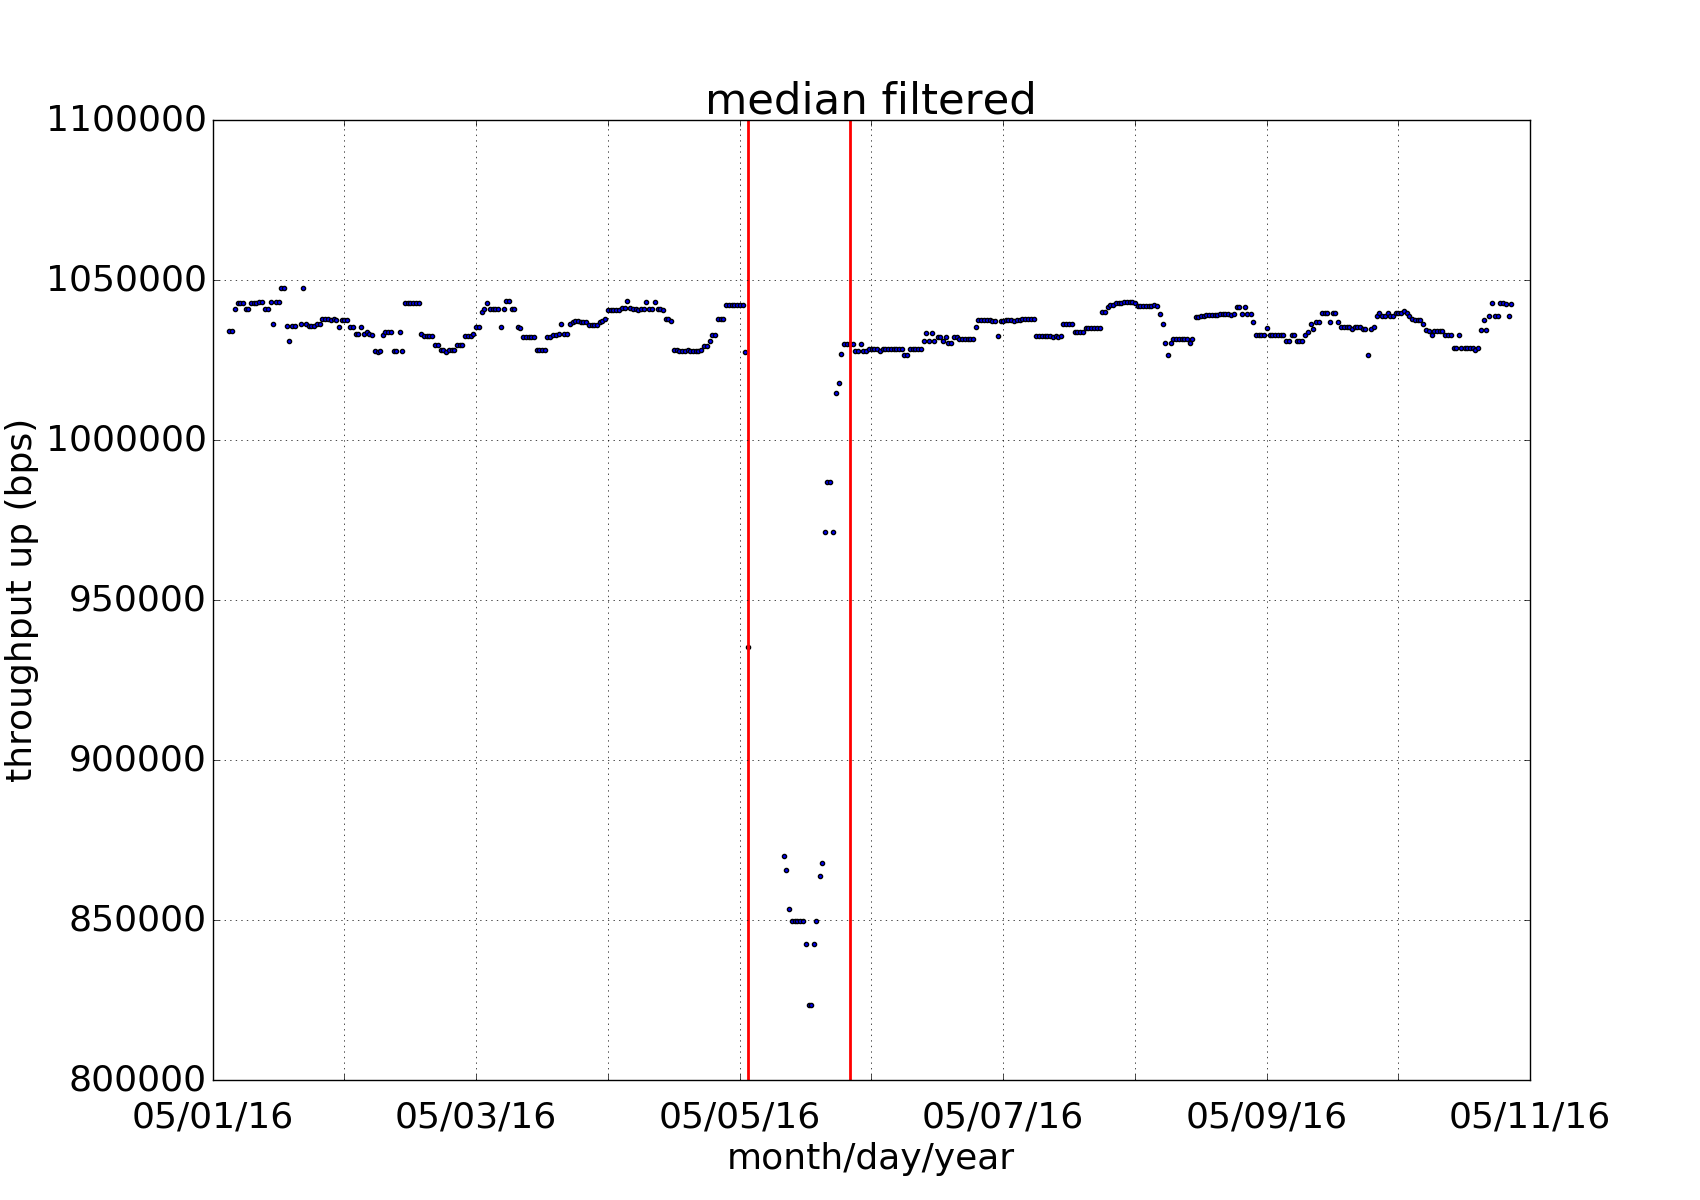
\includegraphics[width=\textwidth]{./figures/results/correct_examples/before_first_hop/serverSDRDTCLDM012_mac64:66:B3:A6:A9:70_dtstart2016-05-01_dtend2016-05-11.png}
            \caption{Client 2.}
        \end{subfigure}%
    }
    \caption{Before first hop.}
\label{fig:before_first_hop}
\end{figure}%

From the 4 clients that belong to this user-group, the system
detected the illustrated events only in these 2 customers.
Then, considering the established suppositions,
these clients must share a physical equipment before the
first hop that caused the events.

Figure~\ref{fig:zero_indegree_correlation_client} shows a client with a
specific network event, and
Figure~\ref{fig:zero_indegree_correlation_user_groups_structure} presents the
user-group structure in which this customer belong.
The vertices are defined by a tuple, in which the first field is a
label to the user-group, and the second specifies the fraction of clients
that detected the considered event.
The gray vertices represent
possible locations resulted from the analysis starting in zero indegree
user-groups.
The blue vertex indicates the correlation between these results.

\begin{figure}[H]
    \centering
    \makebox[\textwidth][c]{%
        \begin{subfigure}[b]{0.45\textwidth}
            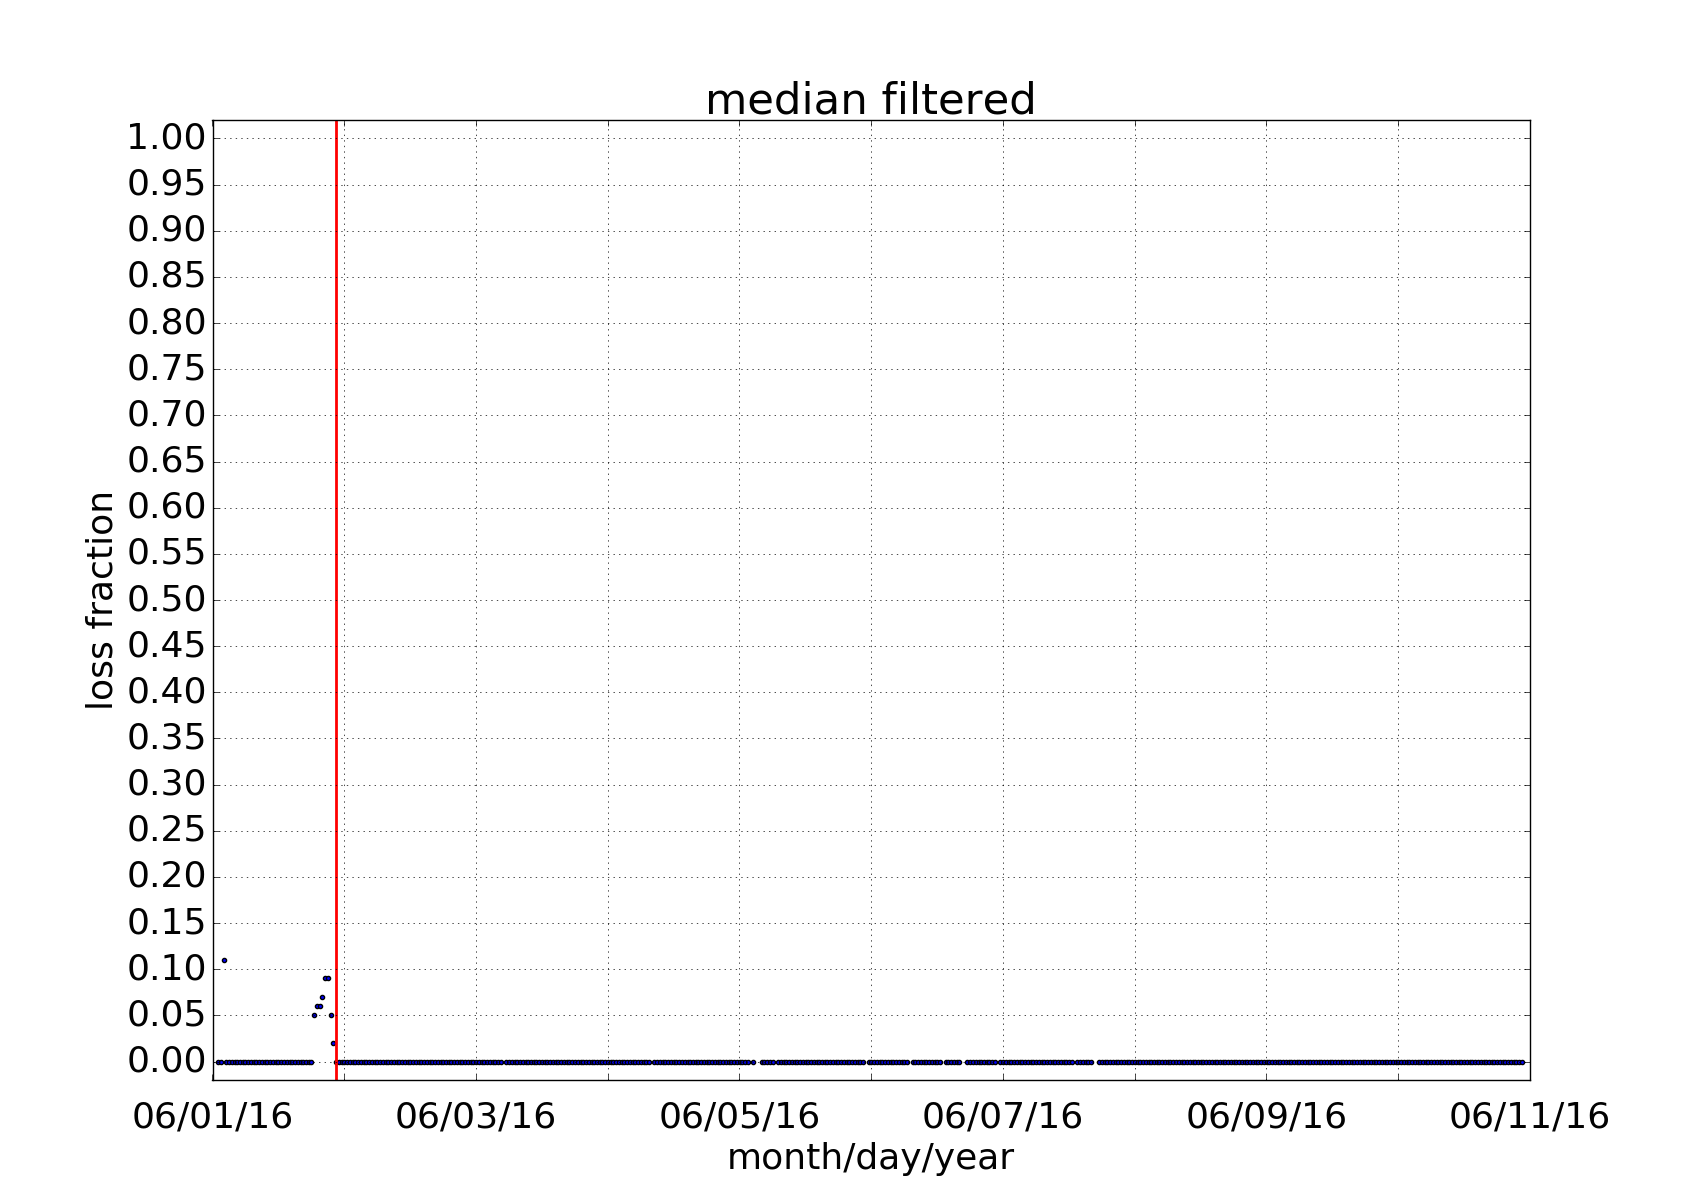
\includegraphics[width=\textwidth]{./figures/results/correct_examples/zero_indegree_correlation/serverSOCDTCPEV01_mac64:66:B3:4F:EA:E2_dtstart2016-06-01_dtend2016-06-11.png}
            \caption{Client 1.}\label{fig:zero_indegree_correlation_client}
        \end{subfigure}
        \begin{subfigure}[b]{0.7\textwidth}
            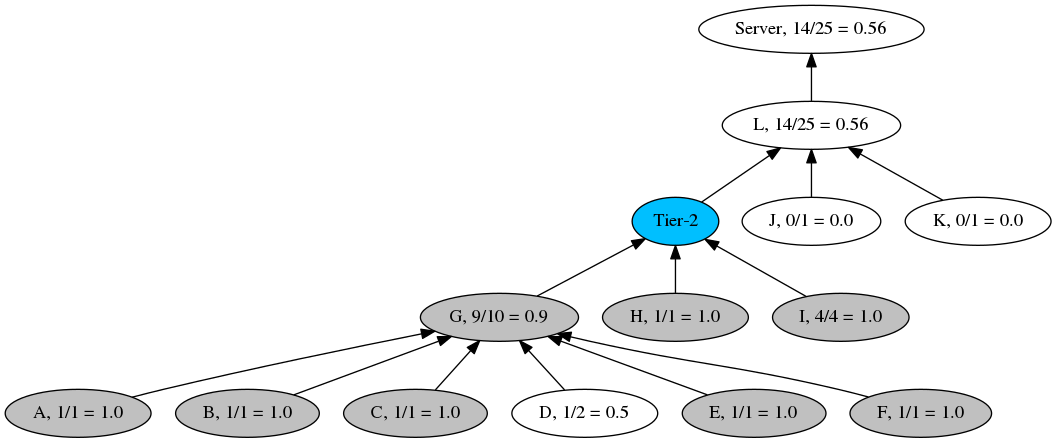
\includegraphics[width=\textwidth]{./figures/results/correct_examples/zero_indegree_correlation/dtstart2016-06-01_dtend2016-06-11_SOCDTCPEV01_traceroute_compress_embratel_graph_anonymized.png}
            \caption{User-groups structure.}\label{fig:zero_indegree_correlation_user_groups_structure}
        \end{subfigure}%
    }
    \caption{Correlation of problem locations detected by analysis that started
    in zero indegree vertices.}
\label{fig:zero_indegreee_correlation}
\end{figure}%

It was visually verified that the same change point pattern of
Figure~\ref{fig:zero_indegree_correlation_client} is present in all clients
that belong to the subtree rooted in the Tier-2 vertex.
Therefore, the system incorrectly did not detect the event in one of the D
user-group clients.
However, since several other G children detected the
event, the system's output was not compromised by this error.
Through the correlation of the zero indegree analysis,
the only match between the problem locations was the Tier-2 group.

Figure~\ref{fig:zero_indegreee_without_correlation} presents an example of a
network event that was only identified in one zero indegree user-group.

\begin{figure}[H]
    \centering
    \makebox[\textwidth][c]{%
        \begin{subfigure}[b]{0.45\textwidth}
            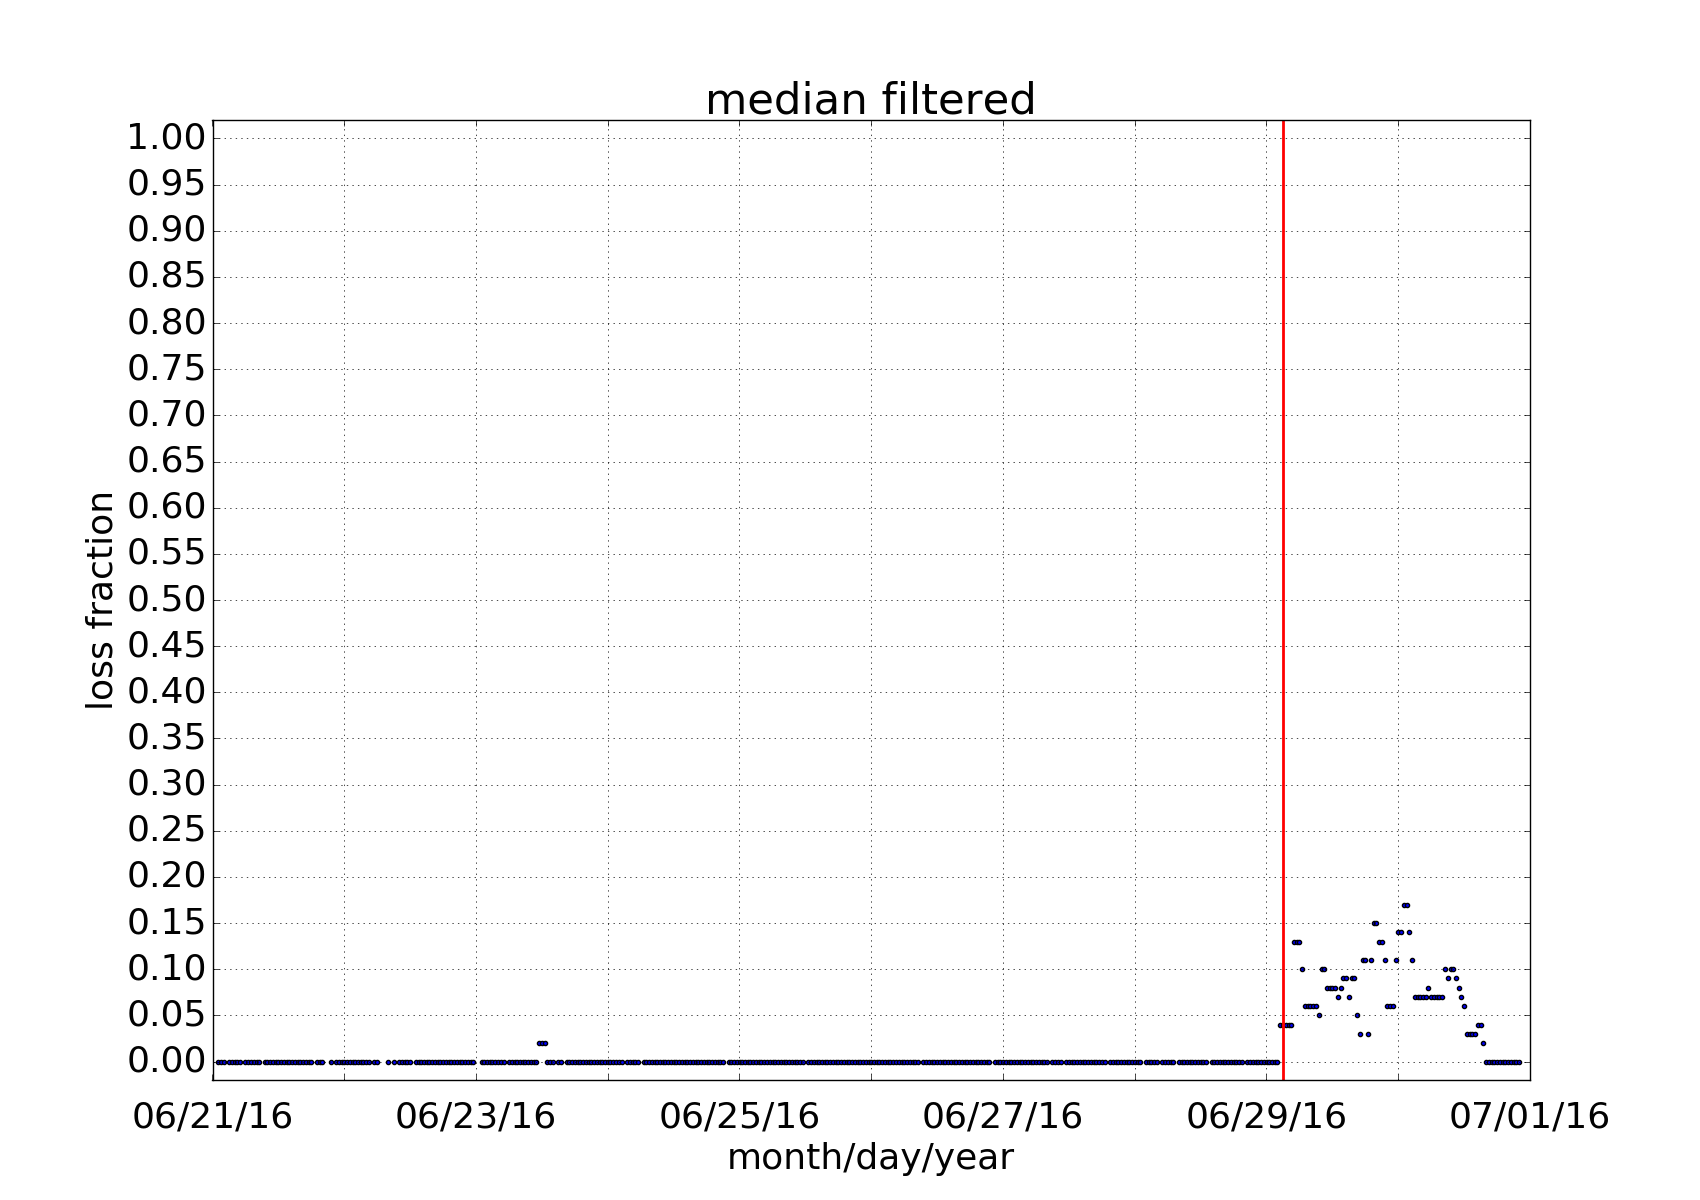
\includegraphics[width=\textwidth]{./figures/results/correct_examples/zero_indegree_single/serverGRSCBCSRV01_mac64:66:B3:50:05:56_dtstart2016-06-21_dtend2016-07-01.png}
            \caption{Client 1.}
        \end{subfigure}
        \begin{subfigure}[b]{0.7\textwidth}
            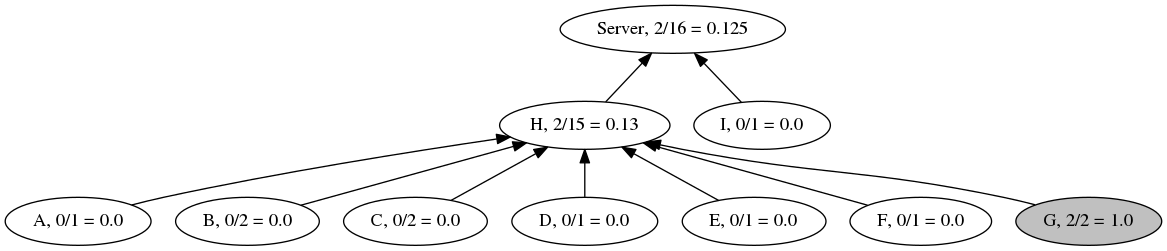
\includegraphics[width=\textwidth]{./figures/results/correct_examples/zero_indegree_single/dtstart2016-06-21_dtend2016-07-01_GRSCBCSRV01_traceroute_compress_embratel_filter_graph_anonymized.png}
            \caption{User-groups structure.}
        \end{subfigure}%
    }
    \caption{Network event in only one zero indegree user-group.}
\label{fig:zero_indegreee_without_correlation}
\end{figure}%

Table~\ref{table:number_of_events} summarizes the number of events considering
the three previous cases. The system didn't detect inconclusive events.

\begin{table}[H]
\centering
\resizebox{\textwidth}{!}{
\begin{tabular}{|c|c|c|c|c|c|c|}
\hline
\multirow{3}{*}{Metric}                & \multicolumn{6}{c|}{Events}                                                                                                                                                                                                                \\ \cline{2-7}
                                       & \multicolumn{2}{c|}{Before first hop} & \multicolumn{2}{c|}{\begin{tabular}[c]{@{}c@{}}Only one zero \\ indegree user-group\end{tabular}} & \multicolumn{2}{c|}{\begin{tabular}[c]{@{}c@{}}Multiple one degree\\ user-groups\end{tabular}} \\ \cline{2-7}
                                       & Improvement         & Failure         & Improvement                                       & Failure                                       & Improvement                                      & Failure                                     \\ \hline
RTT                                    & 688                 & 685             & 789                                               & 809                                           & 43                                               & 38                                          \\ \hline
Round trip loss fraction               & 167                 & 144             & 141                                               & 116                                           & 2                                                & 2                                           \\ \hline
Maximum achievable upstream throughput & 395                 & 358             & 331                                               & 280                                           & 4                                                & 3                                           \\ \hline
\end{tabular}
}
\caption{Number of events.}
\label{table:number_of_events}
\end{table}

\section{Possible Incorrect Outcomes}
\label{sec:possible_wrong_outcomes}

Figure~\ref{fig:time_correlation_unmatch} shows two clients that belong to
the same zero indegree user-group.

\begin{figure}[H]
    \centering
    \makebox[\textwidth][c]{%
        \begin{subfigure}[b]{0.55\textwidth}
            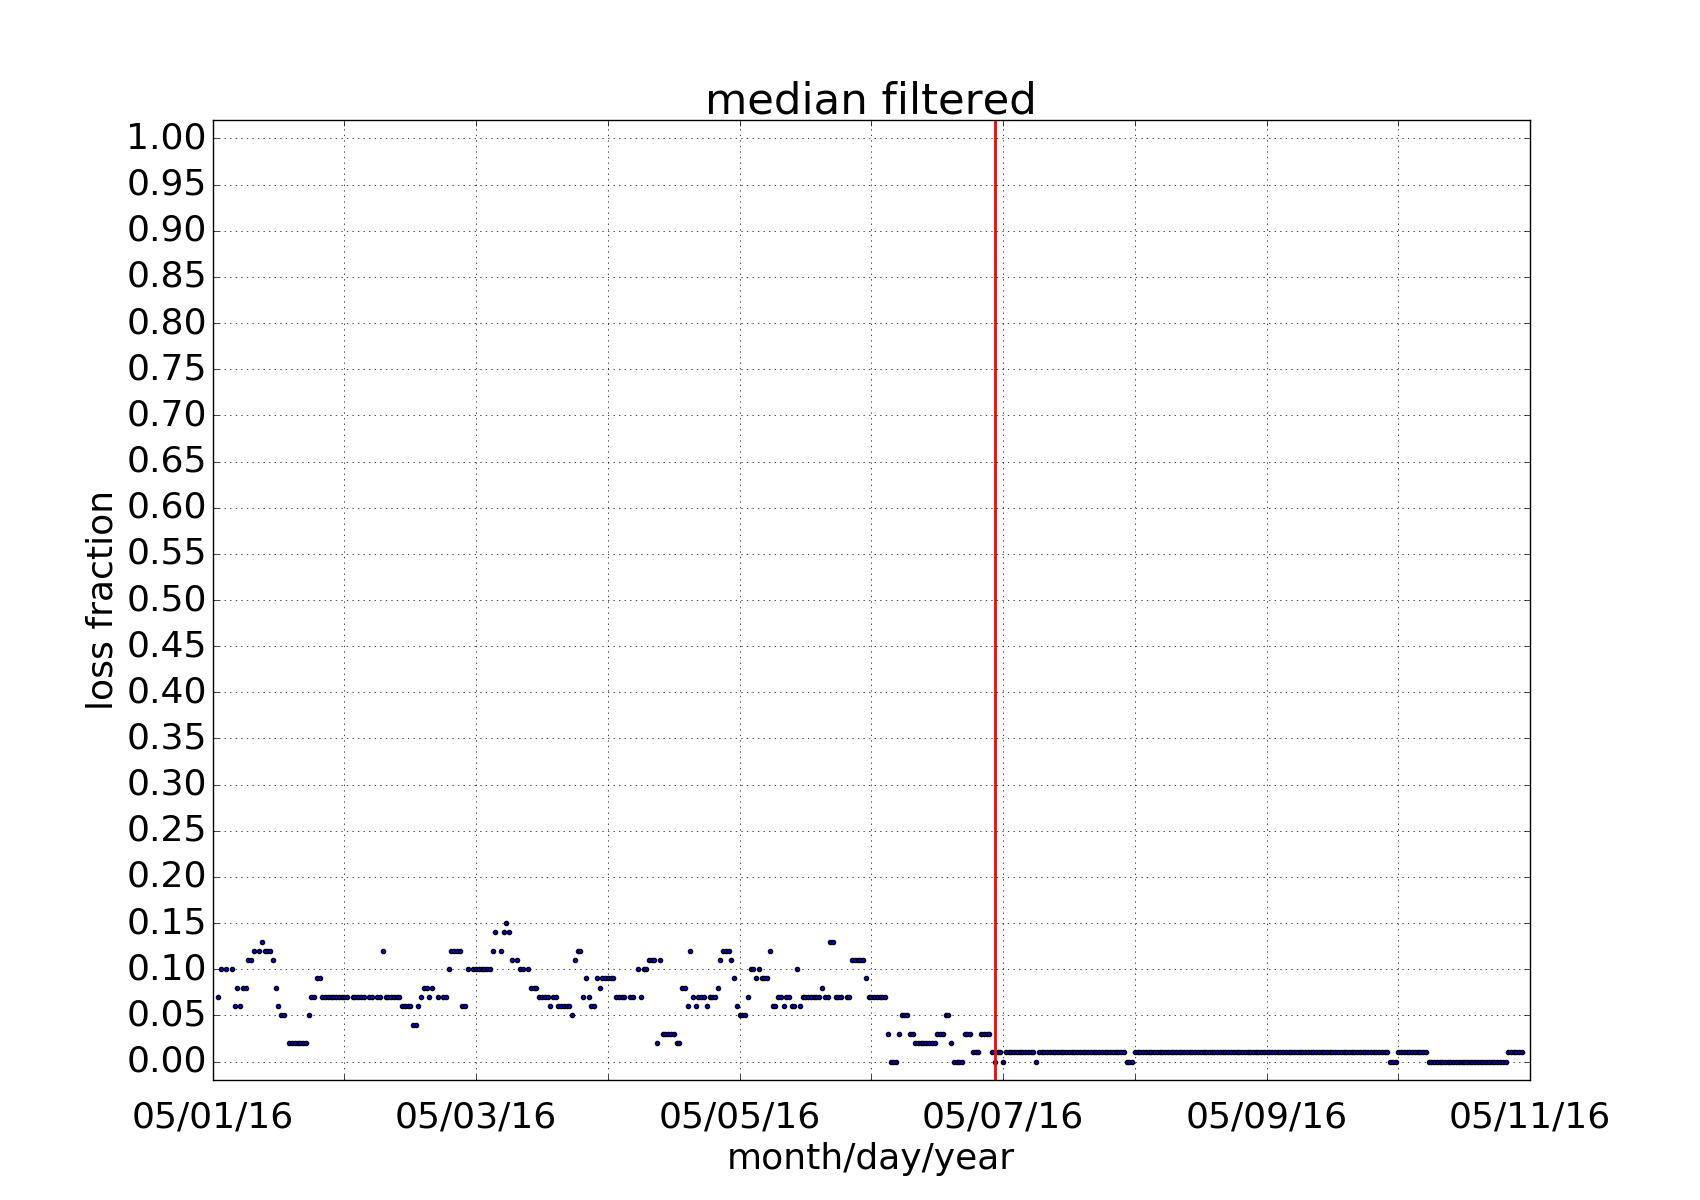
\includegraphics[width=\textwidth]{./figures/results/wrong_examples/time_correlation_example/serverSPOTVTSRV16_mac64:66:B3:A6:AB:80_dtstart2016-05-01_dtend2016-05-11.png}
            \caption{Client 1.}\label{fig:time_correlation_unmatch_client1}
        \end{subfigure}
        \begin{subfigure}[b]{0.55\textwidth}
            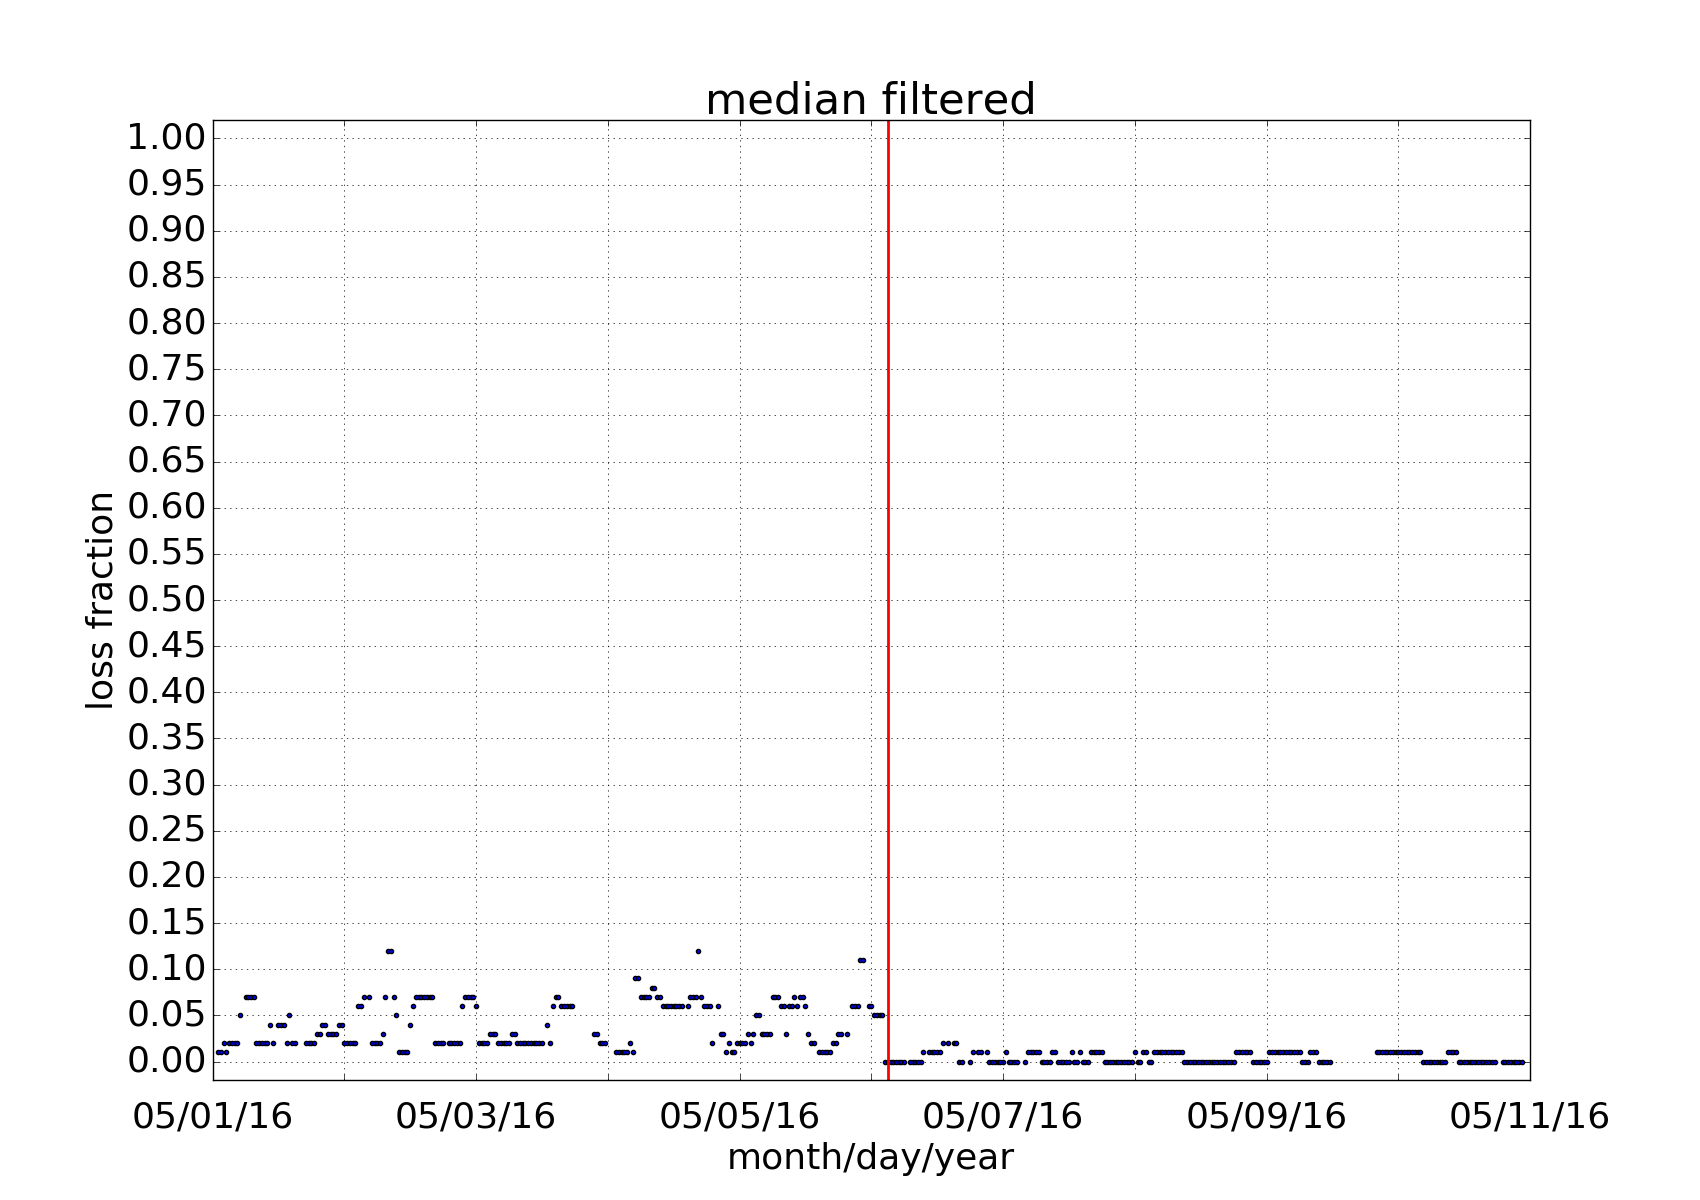
\includegraphics[width=\textwidth]{./figures/results/wrong_examples/time_correlation_example/serverSPOTVTSRV16_mac64:66:B3:A6:AC:40_dtstart2016-05-01_dtend2016-05-11.png}
            \caption{Client 2.}\label{fig:time_correlation_unmatch_client2}
        \end{subfigure}%
    }
    \caption{Time correlation unmatch.}
\label{fig:time_correlation_unmatch}
\end{figure}%

Visually, both time series have similar patterns.
However, in the left client, the change point was detected near the end of
05/07/16 day, and in the right customer, the change was identified in the
beginning of the same day.
All 17 clients of this zero indegree vertex belong to one of these two cases.
Considering the used $\delta$ value, the system recognized two different
events, nonetheless, these changes are possibly related to a single event.
This exemplifies the problem difficulty when there isn't a ground truth,
and also the importance of the algorithms and their hyperparameters selection.
Such kind of subjectivity is usual in the current dataset.

Figure~\ref{fig:untraceable_location} shows two clients that belong to the same
zero indegree vertex.

\begin{figure}[H]
    \centering
    \makebox[\textwidth][c]{%
        \begin{subfigure}[b]{0.55\textwidth}
            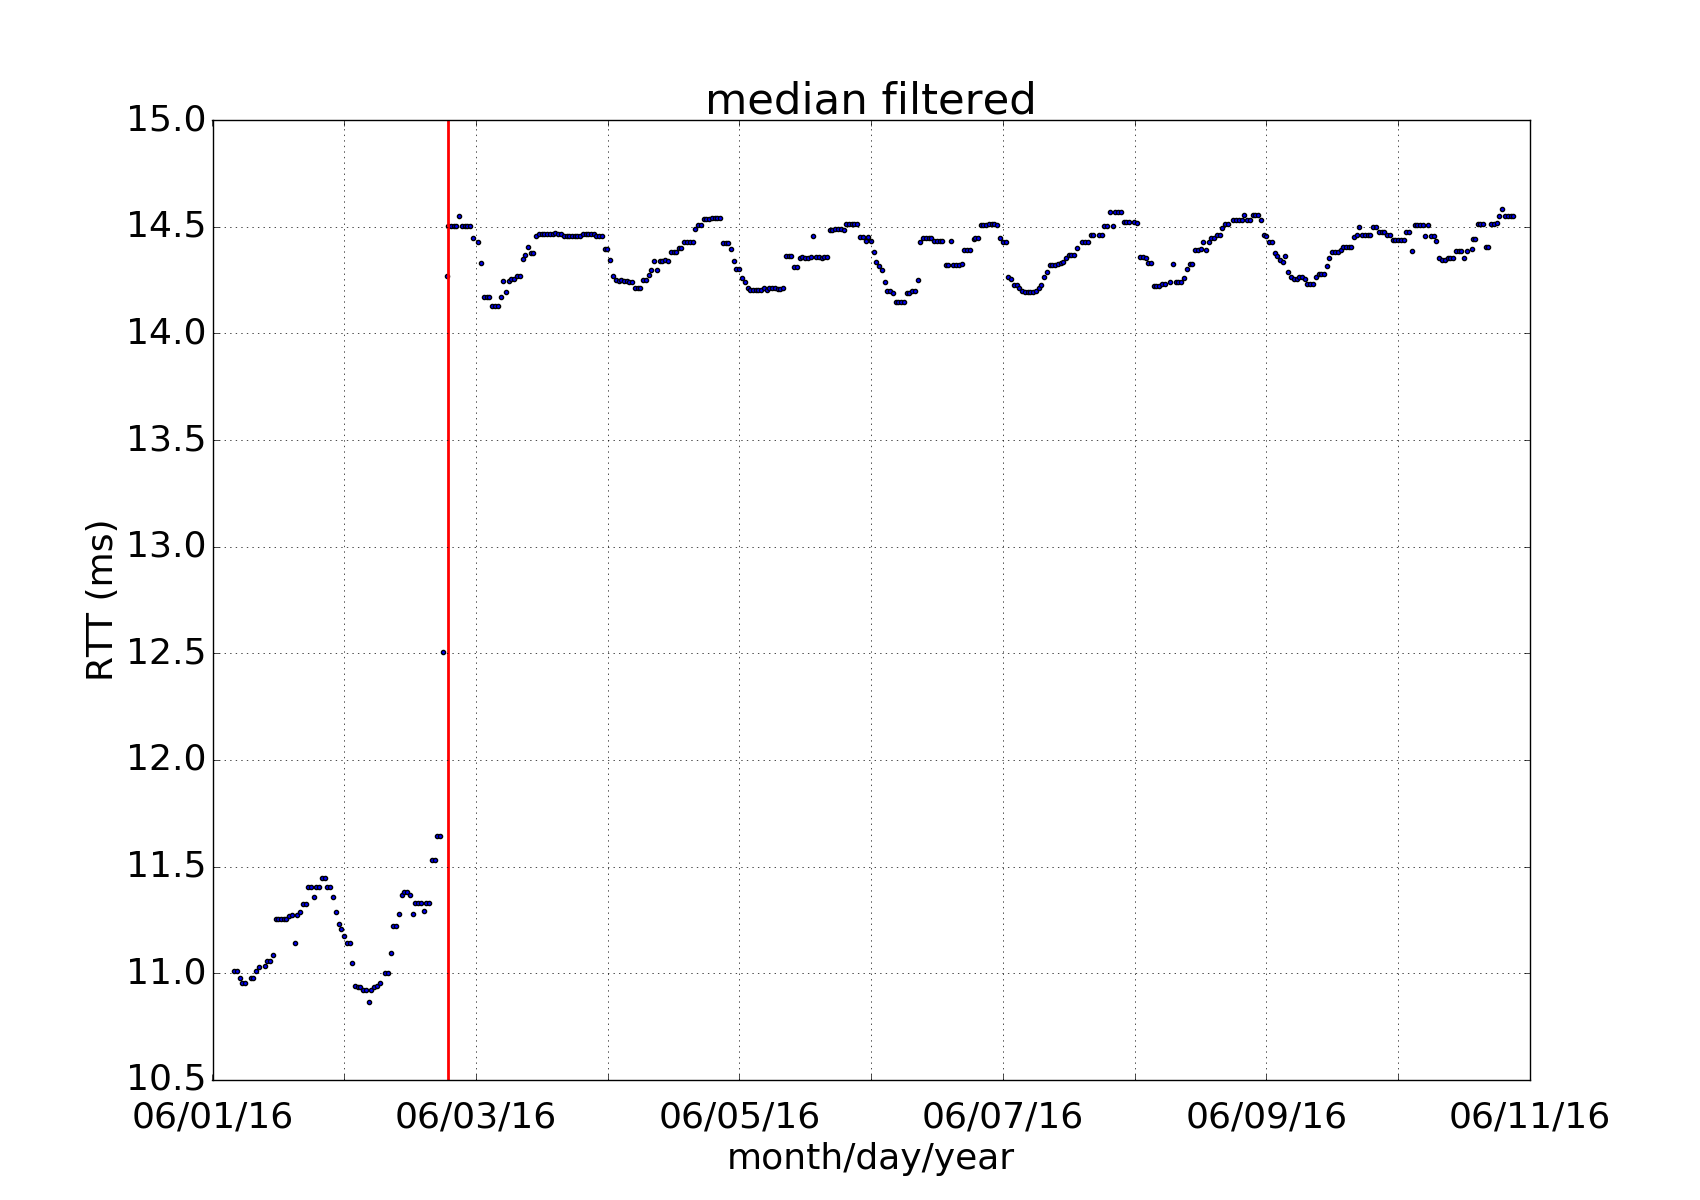
\includegraphics[width=\textwidth]{./figures/results/wrong_examples/untraceable_example/serverBHZDTCLDM062_mac64:66:B3:50:00:68_dtstart2016-06-01_dtend2016-06-11.png}
            \caption{Client 1.}\label{fig:untraceable_location_client_1}
        \end{subfigure}
        \begin{subfigure}[b]{0.55\textwidth}
            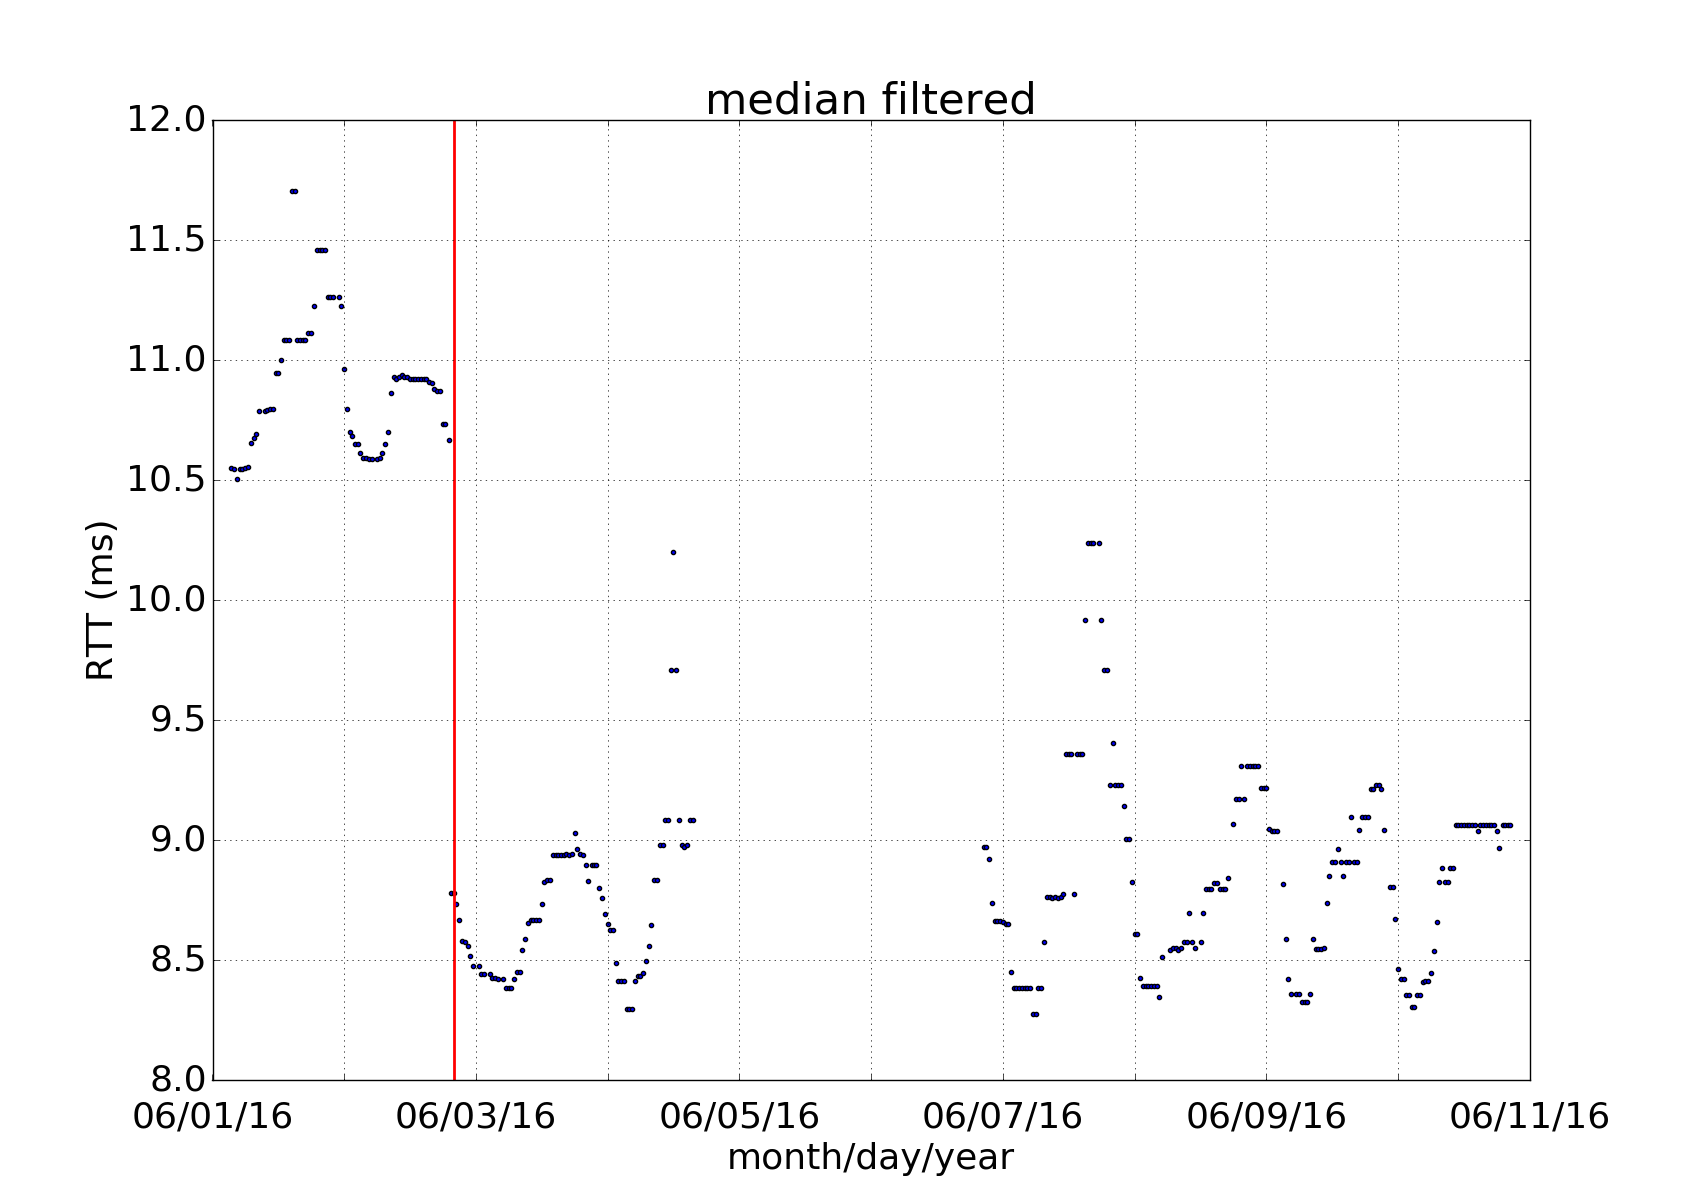
\includegraphics[width=\textwidth]{./figures/results/wrong_examples/untraceable_example/serverBHZDTCLDM062_mac64:66:B3:50:00:B6_dtstart2016-06-01_dtend2016-06-11.png}
            \caption{Client 2.}\label{fig:untraceable_location_client_2}
        \end{subfigure}%
    }
    \caption{Untraceable location.}
\label{fig:untraceable_location}
\end{figure}%

It is possible to note that both RTT time series changed their pattern
nearly at the same time, however, one case is characterized by an improvement,
while the other as a failure.
The traffic between these customers and the server
doesn't go to through the Tier-2 \gls*{isp}, therefore, according with the
suppositions, these patterns indicate simultaneous events that occurred at
different equipments before the first hop.
Nonetheless, the system detected the same RTT modifications, at the end of
06/01/16, in several other clients.
Comparing these customers, it was verified that many of them don't share
several attributes.
For instance, they executed measurements against different servers, their
upstream traffic went to completely different IP layer equipments, and they
were located at different Brazilian UFs.
This can indicate a single global network event, that simultaneously affected
different network regions. As an example, the event could be a centralized
change of \gls*{docsis}' parameters, that is concurrently propagated to all customers.
As with local events, this work doesn't have access to this kind of
information, however, it is intriguing the fact that some of the clients
detected a failure while others perceived an improvement.
It was manually identified 3 of such cases,
and the RTT was the only impacted metric.
A significant number of RTT events were possibly wrongly classified due to this
type of event.

In general, the RTT per hop, obtained through the traceroute measurements,
can be fairly different from the analyzed RTT measures.
First, their methodologies are remarkably distinct.
Second, the RTT associated with hop $i$ can be
constantly and considerably bigger then the RTT related to a hop $j$,
where $j > i$.
This can be explained by the fact that some routers prioritizes
forwarding instead of answering ping packets.
Therefore, the analysis of this data was not included in the framework.
For instance, Figure~\ref{fig:rtt_per_hop_client_1}
presents the RTT per hop, disregarding the server hop, of the client of
Figure~\ref{fig:untraceable_location_client_1}.

\begin{figure}[H]
    \centering
    \makebox[\textwidth][c]{%
        \begin{subfigure}[b]{0.55\textwidth}
            \includegraphics[width=\textwidth]{{./figures/results/wrong_examples/untraceable_example/rtt_per_hop/64:66:B3:50:00:68/hop00_b3ea1801.virtua.com.br}.png}
            \caption{Hop 1}\label{fig:hop_1_client_1}
        \end{subfigure}
        \begin{subfigure}[b]{0.55\textwidth}
            \includegraphics[width=\textwidth]{{./figures/results/wrong_examples/untraceable_example/rtt_per_hop/64:66:B3:50:00:68/hop01_b3ea0001.virtua.com.br}.png}
            \caption{Hop 2}\label{fig:hop_2_client_1}
        \end{subfigure}
    }
    \makebox[\textwidth][c]{%
        \begin{subfigure}[b]{0.55\textwidth}
            \includegraphics[width=\textwidth]{{./figures/results/wrong_examples/untraceable_example/rtt_per_hop/64:66:B3:50:00:68/hop02_c911a615.virtua.com.br}.png}
            \caption{Hop 3}\label{fig:hop_3_client_1}
        \end{subfigure}
        \begin{subfigure}[b]{0.55\textwidth}
            \includegraphics[width=\textwidth]{{./figures/results/wrong_examples/untraceable_example/rtt_per_hop/64:66:B3:50:00:68/hop03_c91180fe.virtua.com.br}.png}
            \caption{Hop 4}\label{fig:hop_4_client_1}
        \end{subfigure}
    }
    \caption{RTT per hop of client of
    Figure~\ref{fig:untraceable_location_client_1}.}
\label{fig:rtt_per_hop_client_1}
\end{figure}%

It is not possible to visually identify the same change pattern of
Figure~\ref{fig:untraceable_location_client_1} in the hops analysis.
Figure~\ref{fig:rtt_per_hop_client_2} is analogous, however, related to client
of Figure~\ref{fig:untraceable_location_client_2}.

\begin{figure}[H]
    \centering
    \makebox[\textwidth][c]{%
        \begin{subfigure}[b]{0.55\textwidth}
            \includegraphics[width=\textwidth]{{./figures/results/wrong_examples/untraceable_example/rtt_per_hop/64:66:B3:50:00:B6/hop00_b3ea1801.virtua.com.br}.png}
            \caption{Hop 1}\label{fig:hop_1_client_2}
        \end{subfigure}
        \begin{subfigure}[b]{0.55\textwidth}
            \includegraphics[width=\textwidth]{{./figures/results/wrong_examples/untraceable_example/rtt_per_hop/64:66:B3:50:00:B6/hop01_b3ea0001.virtua.com.br}.png}
            \caption{Hop 2}\label{fig:hop_2_client_2}
        \end{subfigure}
    }
    \makebox[\textwidth][c]{%
        \begin{subfigure}[b]{0.55\textwidth}
            \includegraphics[width=\textwidth]{{./figures/results/wrong_examples/untraceable_example/rtt_per_hop/64:66:B3:50:00:B6/hop02_c911a615.virtua.com.br}.png}
            \caption{Hop 3}\label{fig:hop_3_client_2}
        \end{subfigure}
        \begin{subfigure}[b]{0.55\textwidth}
            \includegraphics[width=\textwidth]{{./figures/results/wrong_examples/untraceable_example/rtt_per_hop/64:66:B3:50:00:B6/hop03_c91180fe.virtua.com.br}.png}
            \caption{Hop 4}\label{fig:hop_4_client_2}
        \end{subfigure}
    }
    \caption{RTT per hop of client of
    Figure~\ref{fig:untraceable_location_client_2}.}
\label{fig:rtt_per_hop_client_2}
\end{figure}%

In this case, it can be noticed that the RTT is bigger in the beginning of the
first hop time series.
This same pattern was detected in the RTT between the client and the server.

\section{Final Remarks}

Various events related to the maximum achievable upstream
throughput, consist of a substantial mean increase perceived by a single client,
as is exemplified in Figure~\ref{fig:throughput_up_increase}.
Possibly this type of event indicates a change in the customer's contracted
bandwidth.

\begin{figure}[H]
    \centering
    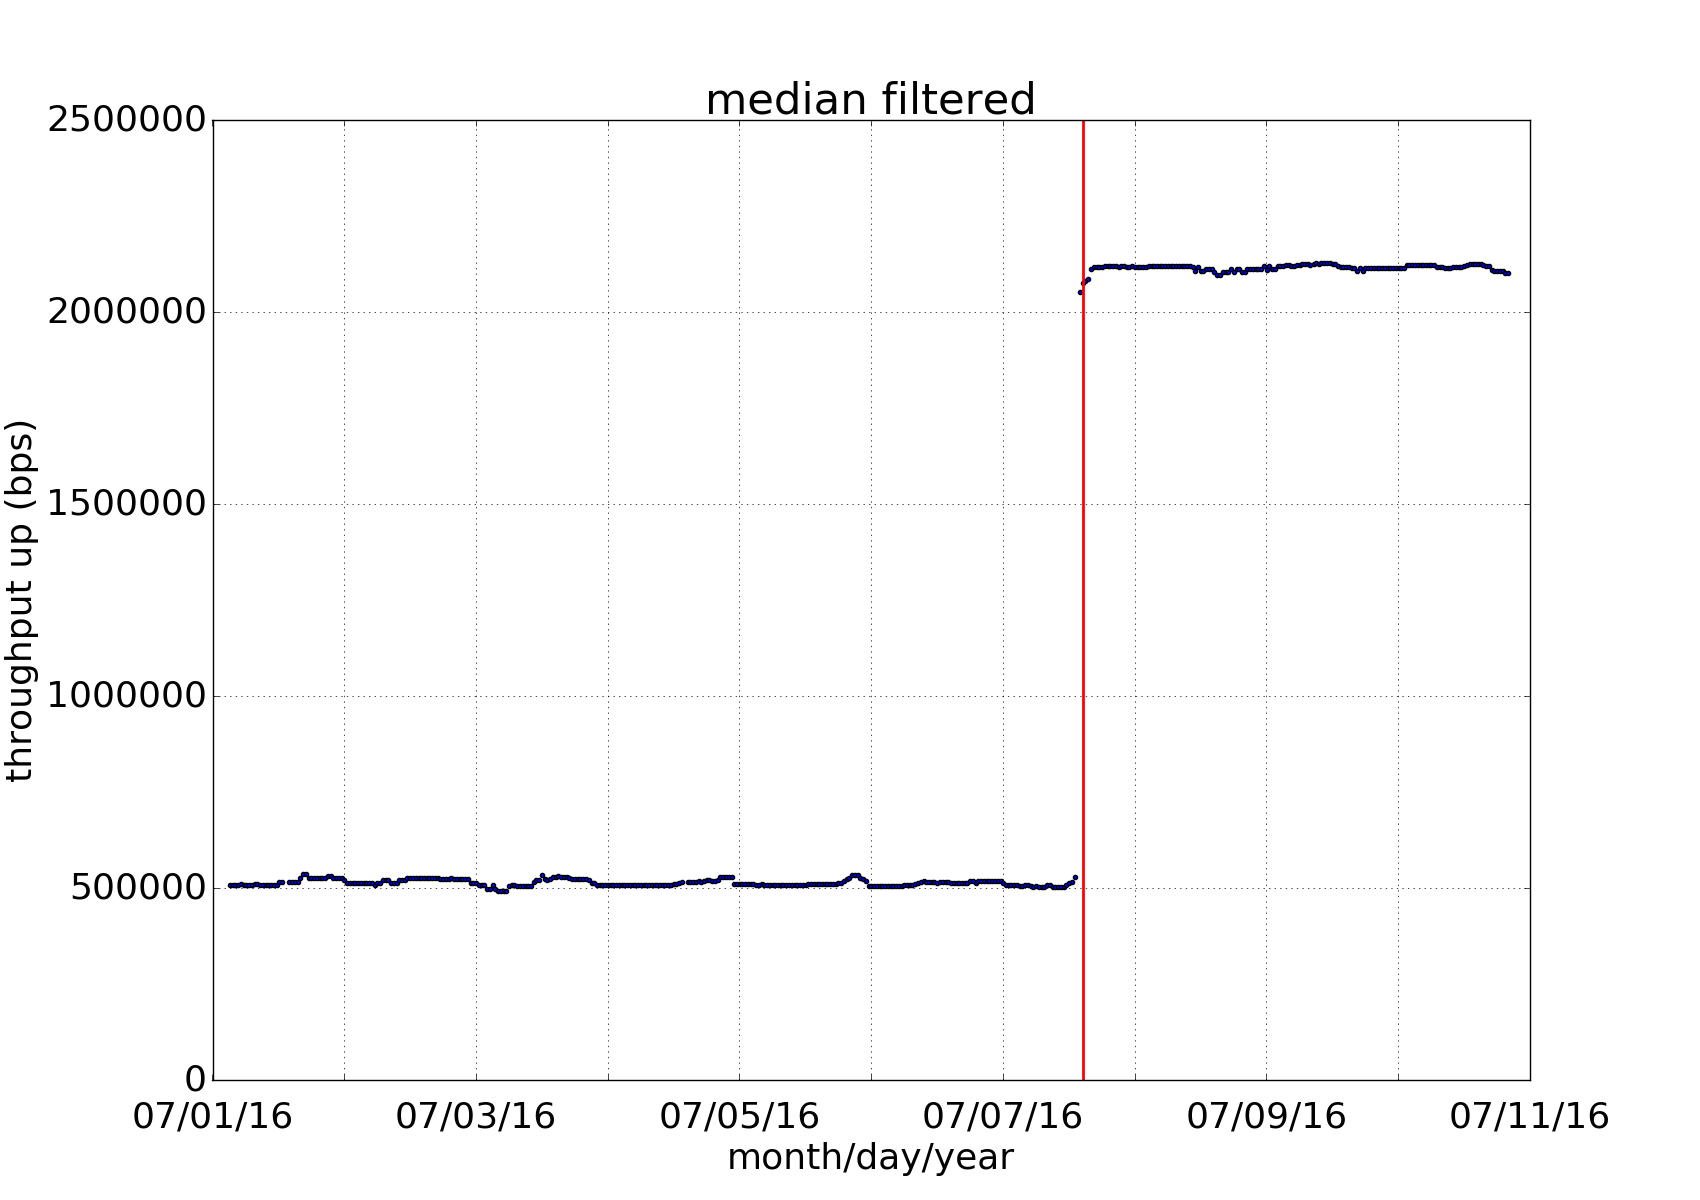
\includegraphics[width=0.7\linewidth]{./figures/results/final_remarks/change_contracted_bandwidth/serverGOIDTCSRV07_macF8:1A:67:2E:E4:9A_dtstart2016-07-01_dtend2016-07-11.png}
    \caption{Possible contract bandwidth change.}
\label{fig:throughput_up_increase}
\end{figure}%

Several problem locations are supported by a change point detected in a single
client.
Figure~\ref{fig:clients_sparsity} exhibits an example.

\begin{figure}[H]
    \centering
    \makebox[\textwidth][c]{%
        \begin{subfigure}[b]{0.45\textwidth}
            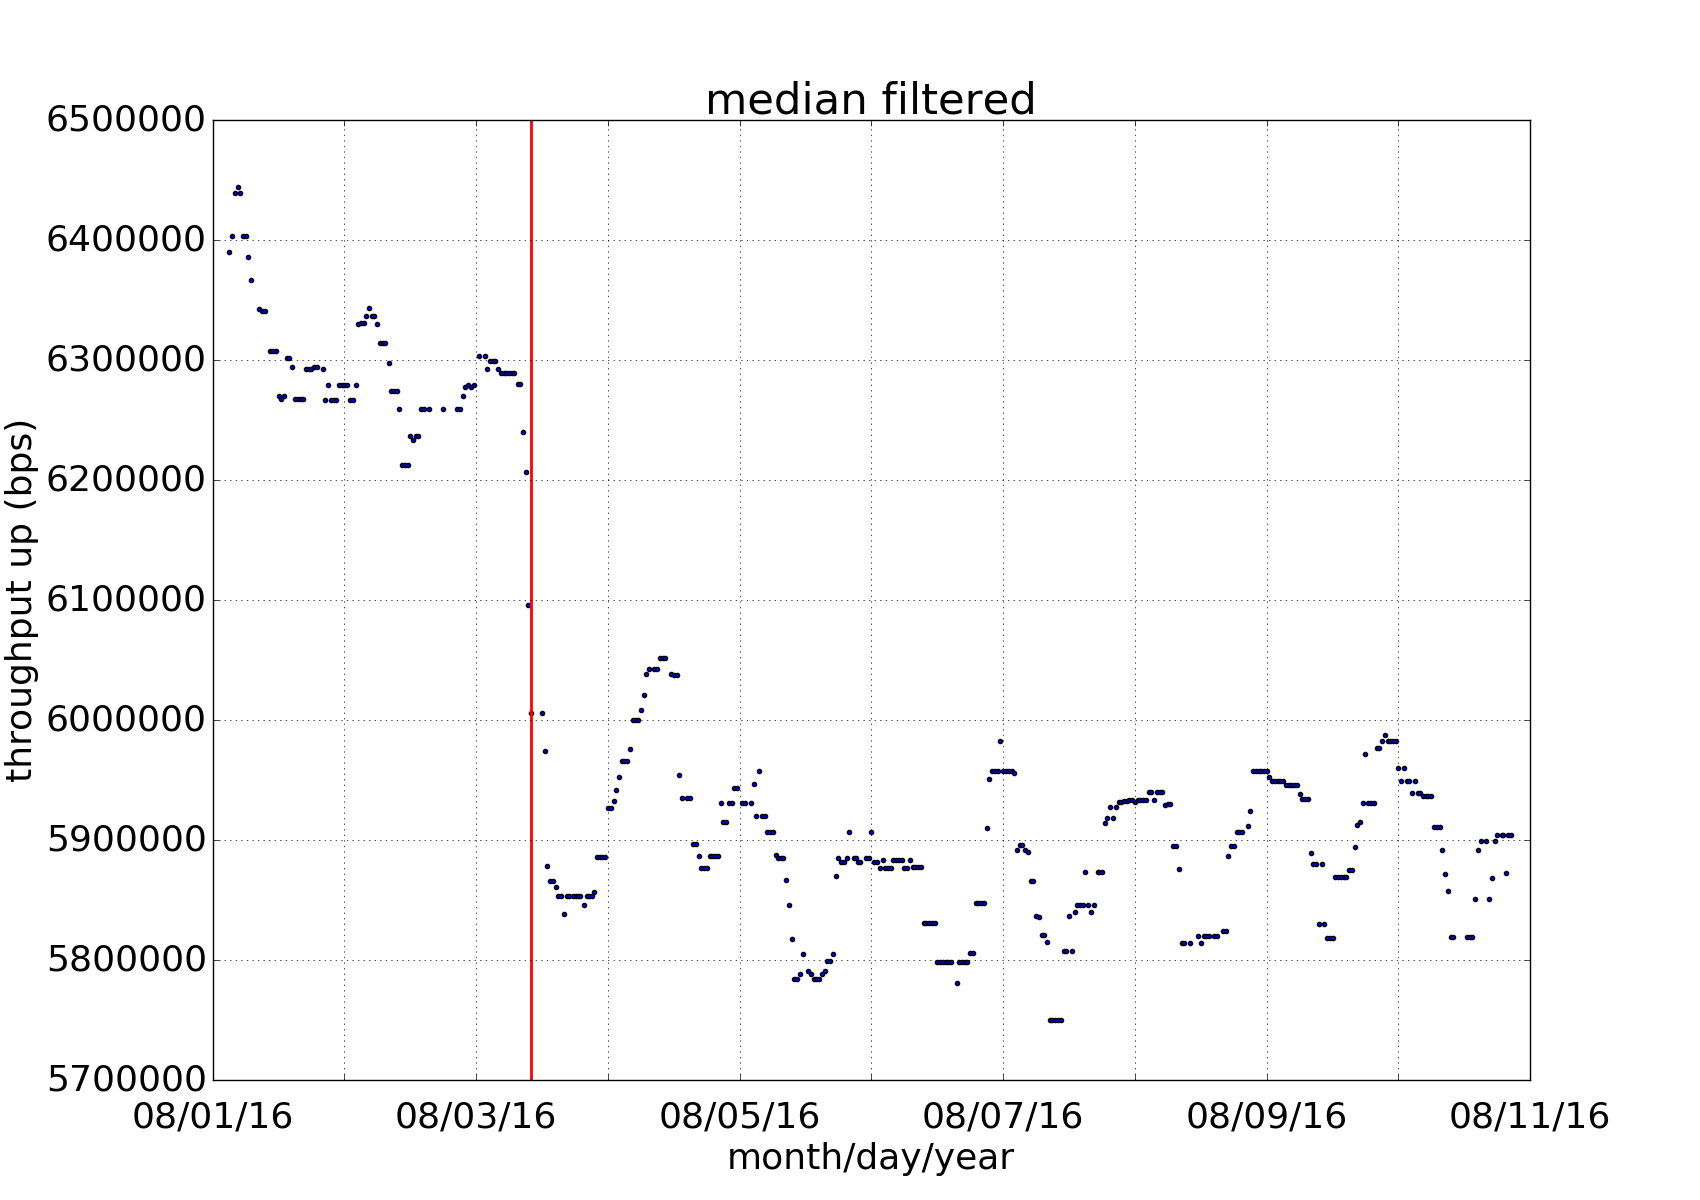
\includegraphics[width=\textwidth]{./figures/results/final_remarks/client_sparsity/serverRJODTCLDM031_mac64:66:B3:4F:E9:24_dtstart2016-08-01_dtend2016-08-11.png}
            \caption{Client 1.}
        \end{subfigure}
        \begin{subfigure}[b]{0.7\textwidth}
            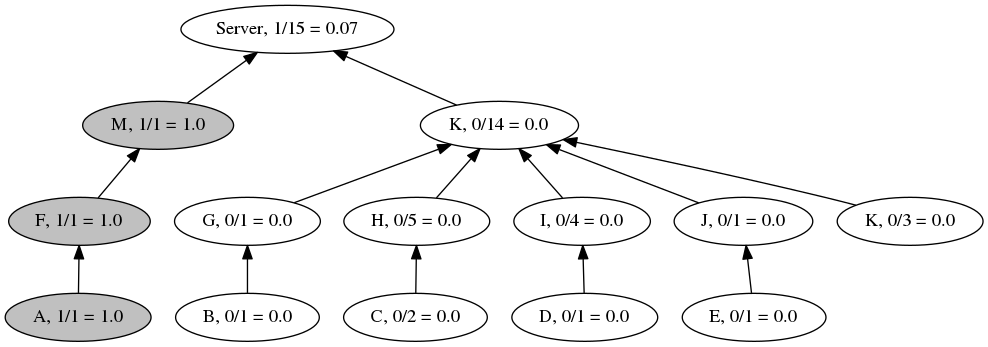
\includegraphics[width=\textwidth]{./figures/results/final_remarks/client_sparsity/dtstart2016-08-01_dtend2016-08-11_RJODTCLDM031_traceroute_compress_embratel_filter_subgraph_anonymized.png}
            \caption{User-groups structure.}
        \end{subfigure}%
    }
    \caption{Clients sparsity.}
\label{fig:clients_sparsity}
\end{figure}%

It is not possible to exactly locate the event,
since the three gray vertices are composed by the same end-user.
This can be avoided with an appropriate selection of the tracked customers.
For instance,
Figure~\ref{fig:number_of_clients_per_zero_indegree_vertex} presents
the number of clients per zero indegree vertex histogram.
More than 70\% of the zero indegree vertices have only one client.

\begin{figure}[H]
    \centering
    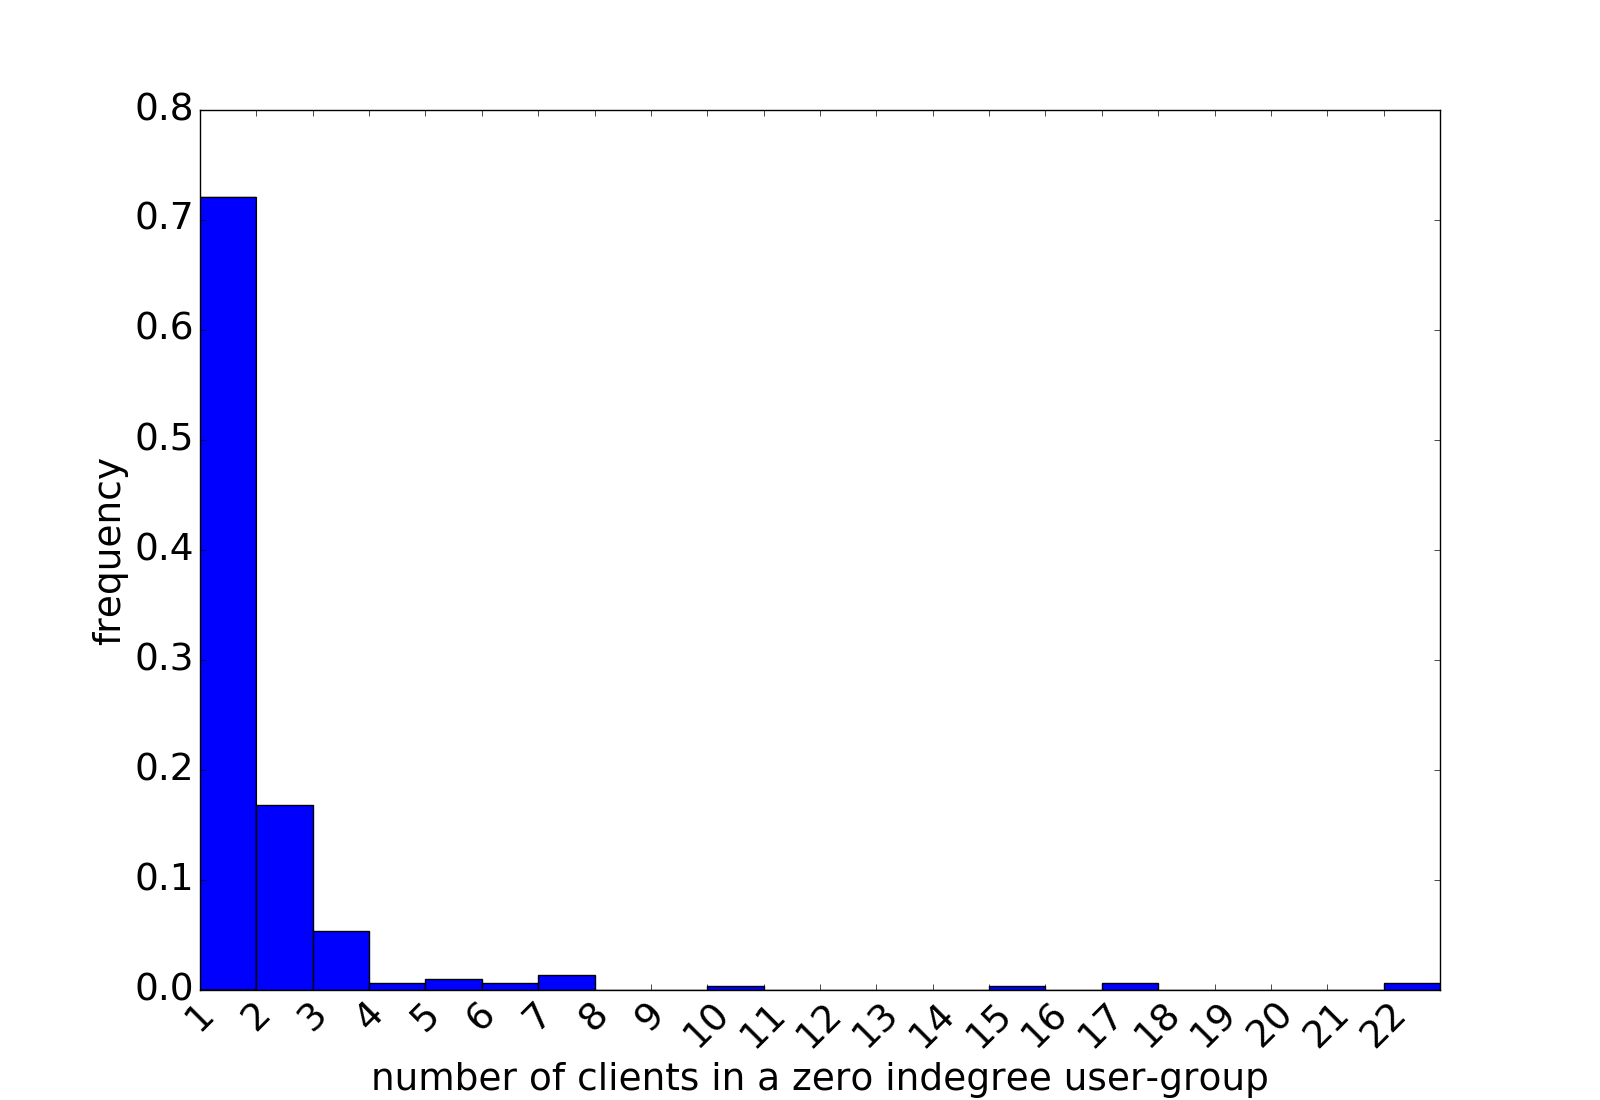
\includegraphics[width=0.7\linewidth]{./figures/results/final_remarks/cnt_clients_zero_indegree_vertex_distribution.png}
    \caption{Number of clients per zero indegree user-group histogram.}
\label{fig:number_of_clients_per_zero_indegree_vertex}
\end{figure}%

    \chapter{Conclusions}
\label{chap:conclusion}

Considering the specific \gls*{isp}'s topology, and the current end-to-end measurement
methodology, this dissertation proposes a data analytics framework to
detect and localize network events.
For such purpose, the mechanism tracks
statistical changes in the end-to-end \gls*{qos} time series from different clients,
and correlates these patterns with traceroutes.
Finally, several outcomes were presented when the procedure was applied to
real data.

The results show that, considering the exposed restrictions,
it is possible to use only end-to-end \gls*{qos} metrics, and traceroutes, from
different clients, to identify and localize network events.
However, due to the lack of an events dataset ground truth, important
questions persist unanswered.
For instance, a quantitative accuracy study
would allow to check which types of events can't be handled by the
proposed mechanism.
A dataset would also allow a precise analysis of the events
patterns, how they impact the \gls*{qos} metrics, and fine tune the system.

The use of end-to-end measurements has the advantage of dealing with
metrics that are directly related with the service perceived by the customers.
As an example, this feature can be used to rank simultaneous failure events
according with their impact to the end-users.
Nonetheless, would be interesting to study the impact of introducing
internal network information to the framework.

Besides the data availability, the current measurement process imposed
several restrictions to this work.
In order to better explore the proposed solution,
a further continuation of this project
would require a stronger partnership with the \gls*{isp}.
In addition, in order to improve the proposed framework's performance,
it would be desirable to adapt the measurement software.
However, this dissertation can be used as a first guide to the \gls*{isp}'s engineers.

\section{Contributions}
Next is summarized this dissertation contributions.

\begin{itemize}
\item
An automatic procedure, that only uses the available end-to-end \gls*{qos}
measurements, and traceroutes, to detect and localize network events in the
specific tier-3 ISP's infrastructure.

\item
A list of possible improvements in the measurement methodology currently
employed by the startup, in order to enhance the proposed system's performance. This
list is presented in the next Section~\ref{sec:future_work}.
\end{itemize}

\section{Future Work}
\label{sec:future_work}

Next is presented a list of future development directions of this work.
Considering the detection and localization of events, several adaptations to
the current measurement methodology are suggested.

\begin{itemize}
\item
The used \gls*{qos} metrics are affected by equipments in the path from the server to
the end-user, as well as those in the reverse direction.
However, only the path information from end-users to servers are available.
Hence, the traceroutes from servers to end-users should also be collected.
Besides, instead of only considering the round trip loss information,
the one way loss fraction in both directions can be tracked.
Further, the maximum achievable one way throughput measurement can be
implemented using \gls*{udp} instead of \gls*{tcp}, which eliminates the interference of
performance degradation in the reverse path.

\item
The \gls*{hfc} plant between the home router and the
first hop of the traceroute can be incorporated to the analysis.
Also, in addition to only using end-to-end \gls*{qos} metrics,
the proposed mechanism can be extended
to use internal network devices information, such as signal-to-noise ratio.

\item
A network failure events dataset can be built with \gls*{isp}'s data.
As an example, customers' complaints gathered from call centers can be used to,
during a specific time period, infer clients affected by a \gls*{qoe} deterioration,
which can then be translated to true network failures.
Additionally, it is possible to use records from current failure detection
methods deployed by the \gls*{isp}, such as manual inspection, or through equipments
that are able to report specific faults.
However, through preliminary talks with \gls*{isp}'s engineers,
both databases are noisy, and mining useful information
from them can be a challenging task.
For instance, there are cases in which devices flaws are manually
detected and corrected, but those information is not stored.
Also, during the dataset construction, the inferred events times can be
considerably different from their true occurrence time.
As stated in Chapter~\ref{chap:methodology}, a dataset could open new
supervised learning possibilities to the change point detection problem, such
as hyperparameter optimization and model selection.
Besides, since the tier-2 \gls*{isp} is not a project partner, this
complete data of the network infrastructure may not be available.

\item
Once a network events dataset is constructed, the correlation between
change points of different \gls*{qos} metrics can reveal useful information
about the network behavior. This analysis was not done since the algorithms'
hyperparameters couldn't be optimized, hence, these comparisons could reach
wrong conclusions.

\item
A deeper knowledge of the tier-2 \gls*{isp}'s infrastructure
can be used to model the tier-2 network with finer granularity in the Spatial
Correlation procedure, which can improve the system's event localization
precision.

\item
It is planned in the \gls*{isp}'s roadmap to increase the number of tracked customers.
In this case, the system's computational performance can benefit from data
aggregation techniques, as it was done in Argus.
Besides, this increase will naturally improve the internal network equipments
coverage by the end-to-end measurements, which, as the previous topic, can
enhance the events localization precision.

\item
Once the system is deployed, the algorithms and parameters can be selected
through a reinforcement learning approach. If network operators
feedback the outcomes' correctness, the system can adaptively optimize the used
strategies.

\item
Considering a real time processing environment, in order to decrease the
event detection delay, the system can adaptively control the measurement
frequency.
Increasing the amount of data related to potentially problematic regions,
can improve the system's output confidence in a short time period.
Also, it is possible to reduce the measurement frequency in well behaved
localities, which can lower the traffic overhead generated by measurements, and
increase the data analytics computational performance.

\item
Instead of centrally process the time series,
it is possible to instrument the home
gateways to detect changes in an online fashion. Then, as with \gls*{cem}, the home
routers could push this information to a central database for further analysis.

\item
Extend the mechanism to deal with other types of network infrastructures.

\end{itemize}


    \backmatter{}
    \nocite{*}
    \bibliographystyle{coppe-unsrt}
    \bibliography{./src/bibliography}

\end{document}
